%%%%%%%%%%%%%%%%%%%%%%%%%%%%% Thesis.tex %%%%%%%%%%%%%%%%%%%%%%%%%%%%%%%
%                                                                      %
%  ---------- Master of Science Dissertation template ----------       %
%                                                                      %
%  Template for the Master Thesis according to the regulations         %
%  published by the Academic Board (Direcção Académica) at IST.        %
%                                                                      %
%  For up-to-date guide, please refer to the offical website           %
%  http://da.tecnico.ulisboa.pt/dissertacao-de-mestrado/               %
%                                                                      %
%       Andre C. Marta                                                 %
%       Area Cientifica de Mecanica Aplicada e Aeroespacial            %
%       Departamento de Engenharia Mecanica                            %
%       Instituto Superior Tecnico                                     %
%       Av. Rovisco Pais                                               %
%       1049-001 Lisboa                                                %
%       Portugal                                                       %
%       Tel: +351 21 841 9469                                          %
%                        3469 (extension)                              %
%       Email: andre.marta@tecnico.ulisboa.pt                          %
%                                                                      %
%  Created:       Jan 20, 2011                                         %
%  Last Modified: Jul  2, 2015                                         %
%                                                                      %
%%%%%%%%%%%%%%%%%%%%%%%%%%%%%%%%%%%%%%%%%%%%%%%%%%%%%%%%%%%%%%%%%%%%%%%%
%  Revision history                                                    %
%  v1 - 2011/01/24 - original template                                 %
%  v2 - 2012/10/30 - new IST image and glossary support                %
%  v3 - 2013/12/10 - update according to 2012/13 official guide        %
%  v4 - 2014/02/28 - new default for bibliography style                %
%  v5 - 2014/05/07 - update according to 2013/14 official guide        %
%  v6 - 2015/07/02 - cover page format fixed,                          %
%                    contents page numbering fixed,                    %
%                    better language support,                          %
%                    enhanced examples of tables,                      %
%                    new option for appendix page numbering format,    %
%                    custom bibliography style                         %
%%%%%%%%%%%%%%%%%%%%%%%%%%%%%%%%%%%%%%%%%%%%%%%%%%%%%%%%%%%%%%%%%%%%%%%%
%                                                                      %
% To generate the PDF file, type "make" at the terminal prompt.        %
%                                                                      %
% The IST template LaTeX package was created by the author             %
% and it can be downloaded from:                                       %
% https://fenix.ist.utl.pt/homepage/ist31052/                          %
%                                                                      %
% The external packages can be downloaded from                         %
% the Comprehensive TeX Archive Network at http://www.ctan.org/        %
%                                                                      %
% List of LaTex symbols:                                               %
% http://www.ctan.org/tex-archive/info/symbols/comprehensive/          %
%                                                                      %
% Help with LaTex can be found at                                      %
% http://www.giss.nasa.gov/tools/latex/ltx-2.html                      %
% http://en.wikibooks.org/wiki/LaTeX                                   %
%%%%%%%%%%%%%%%%%%%%%%%%%%%%%%%%%%%%%%%%%%%%%%%%%%%%%%%%%%%%%%%%%%%%%%%%

%%%%%%%%%%%%%%%%%%%%%%%%%%%%%%%%%%%%%%%%%%%%%%%%%%%%%%%%%%%%%%%%%%%%%%%%
%     Preamble                                                         %
%%%%%%%%%%%%%%%%%%%%%%%%%%%%%%%%%%%%%%%%%%%%%%%%%%%%%%%%%%%%%%%%%%%%%%%%

% ----------------------------------------------------------------------
%  Set the document class
% ----------------------------------------------------------------------
\documentclass[11pt,a4paper,twoside]{report}  %mpc: changed, was 10
\usepackage{listings}
\usepackage{tgpagella}        
\usepackage[scaled=0.85]{beramono} 
\usepackage[T1]{fontenc}     

\usepackage{drawstack}
\usepackage{graphicx}
\usepackage{subcaption}
\usepackage{qtree}
\usepackage{spreadtab}
\usepackage{forest}
\usepackage{makecell}
\setlength\extrarowheight{4pt}

\renewcommand\theadfont{\bfseries}
\renewcommand\theadgape{\Gape[4pt]}
\renewcommand\cellgape{\Gape[4pt]}
% ----------------------------------------------------------------------
% Define external packages, language, margins, fonts and new commands
% ----------------------------------------------------------------------
%%%%%%%%%%%%%%%%%%%%%%%%%%%%%%%%%%%%%%%%%%%%%%%%%%%%%%%%%%%%%%%%%%%%%%%%
%                                                                      %
%     File: Thesis_Preamble.tex                                        %
%     Tex Master: Thesis.tex                                           %
%                                                                      %
%     Author: Andre C. Marta                                           %
%     Last modified : 9 Apr 2015                                       %
%                                                                      %
%%%%%%%%%%%%%%%%%%%%%%%%%%%%%%%%%%%%%%%%%%%%%%%%%%%%%%%%%%%%%%%%%%%%%%%%

% ----------------------------------------------------------------------
% Define document language.
% ----------------------------------------------------------------------

% 'inputenc' package
%
% Accept different input encodings.
% http://www.ctan.org/tex-archive/macros/latex/base/
%
% > allows typing non-english text in LaTeX sources.
%
% ******************************* SELECT *******************************
%\usepackage[latin1]{inputenc} % <<<<< Windows
\usepackage[utf8]{inputenc}   % <<<<< Linux
% ******************************* SELECT *******************************


% 'babel' package
%
% Multilingual support for Plain TeX or LaTeX.
% http://www.ctan.org/tex-archive/macros/latex/required/babel/
%
% > sets the variable names according to the language selected
%
% ******************************* SELECT *******************************
%\usepackage[portuguese]{babel} % <<<<< Portuguese
\usepackage[english]{babel} % <<<<< English
% ******************************* SELECT *******************************


% List of LaTeX variable names: \abstractname, \appendixname, \bibname,
%   \chaptername, \contentsname, \listfigurename, \listtablename, ...)
% http://www.tex.ac.uk/cgi-bin/texfaq2html?label=fixnam
%
% Changing the words babel uses (uncomment and redefine as necessary...)
%
\newcommand{\acknowledgments}{@undefined} % new LaTeX variable name
%
% > English
%
\addto\captionsenglish{\renewcommand{\acknowledgments}{Acknowledgments}}
%\addto\captionsenglish{\renewcommand{\contentsname}{Contents}}
%\addto\captionsenglish{\renewcommand{\listtablename}{List of Tables}}
%\addto\captionsenglish{\renewcommand{\listfigurename}{List of Figures}}
%\addto\captionsenglish{\renewcommand{\nomname}{Nomenclature}}
%\addto\captionsenglish{\renewcommand{\glossaryname}{Glossary}}
%\addto\captionsenglish{\renewcommand{\acronymname}{List of Acronyms}}
%\addto\captionsenglish{\renewcommand{\bibname}{References}} % Bibliography
%\addto\captionsenglish{\renewcommand{\appendixname}{Appendix}}

% > Portuguese
%
\addto\captionsportuguese{\renewcommand{\acknowledgments}{Agradecimentos}}
%\addto\captionsportuguese{\renewcommand{\contentsname}{Conte\'{u}do}}
%\addto\captionsportuguese{\renewcommand{\listtablename}{Lista de Figuras}}
%\addto\captionsportuguese{\renewcommand{\listfigurename}{Lista de Tabelas}}
\addto\captionsportuguese{\renewcommand{\nomname}{Lista de S\'{i}mbolos}} % Nomenclatura
%\addto\captionsportuguese{\renewcommand{\glossary}{Gloss\'{a}rio}}
%\addto\captionsportuguese{\renewcommand{\acronymname}{Lista de Abrevia\c{c}\~{o}es}}
%\addto\captionsportuguese{\renewcommand{\bibname}{Refer\^{e}ncias}} % Bibliografia
%\addto\captionsportuguese{\renewcommand{\appendixname}{Anexo}} % Apendice


% ----------------------------------------------------------------------
% Define cover fields in both english and portuguese.
% ----------------------------------------------------------------------
%
\newcommand{\coverThesis}{@undefined} % new LaTeX variable name
\newcommand{\coverSupervisors}{@undefined} % new LaTeX variable name
\newcommand{\coverExaminationCommittee}{@undefined} % new LaTeX variable name
\newcommand{\coverChairperson}{@undefined} % new LaTeX variable name
\newcommand{\coverSupervisor}{@undefined} % new LaTeX variable name
\newcommand{\coverMemberCommittee}{@undefined} % new LaTeX variable name
% > English
\addto\captionsenglish{\renewcommand{\coverThesis}{Thesis to obtain the Master of Science Degree in}}
\addto\captionsenglish{\renewcommand{\coverSupervisors}{Supervisors}}
\addto\captionsenglish{\renewcommand{\coverExaminationCommittee}{Examination Committee}}
\addto\captionsenglish{\renewcommand{\coverChairperson}{Chairperson}}
\addto\captionsenglish{\renewcommand{\coverSupervisor}{Supervisor}}
\addto\captionsenglish{\renewcommand{\coverMemberCommittee}{Member of the Committee}}
% > Portuguese
\addto\captionsportuguese{\renewcommand{\coverThesis}{Disserta\c{c}\~{a}o para obten\c{c}\~{a}o do Grau de Mestre em}}
\addto\captionsportuguese{\renewcommand{\coverSupervisors}{Orientador(es)}}
\addto\captionsportuguese{\renewcommand{\coverExaminationCommittee}{J\'{u}ri}}
\addto\captionsportuguese{\renewcommand{\coverChairperson}{Presidente}}
\addto\captionsportuguese{\renewcommand{\coverSupervisor}{Orientador}}
\addto\captionsportuguese{\renewcommand{\coverMemberCommittee}{Vogal}}


% ----------------------------------------------------------------------
% Define default and cover page fonts.
% ----------------------------------------------------------------------

% Use Arial font as default
%
%\renewcommand{\rmdefault}{phv}  %mpc: changed, commented these 2 lines; Arial doesn't look good
%\renewcommand{\sfdefault}{phv}

% Define cover page fonts
%
%         encoding     family       series      shape
%  \usefont{T1}     {phv}=helvetica  {b}=bold    {n}=normal
%                   {ptm}=times      {m}=normal  {sl}=slanted
%                                                {it}=italic
% see more examples at
% http://julien.coron.free.fr/languages/latex/fonts/
%
\def\FontLn{% 16 pt normal
  \usefont{T1}{phv}{m}{n}\fontsize{16pt}{16pt}\selectfont}
\def\FontLb{% 16 pt bold
  \usefont{T1}{phv}{b}{n}\fontsize{16pt}{16pt}\selectfont}
\def\FontMn{% 14 pt normal
  \usefont{T1}{phv}{m}{n}\fontsize{14pt}{14pt}\selectfont}
\def\FontMb{% 14 pt bold
  \usefont{T1}{phv}{b}{n}\fontsize{14pt}{14pt}\selectfont}
\def\FontSn{% 12 pt normal
  \usefont{T1}{phv}{m}{n}\fontsize{12pt}{12pt}\selectfont}


% ----------------------------------------------------------------------
% Define page margins and line spacing.
% ----------------------------------------------------------------------

% 'geometry' package
%
% Flexible and complete interface to document dimensions.
% http://www.ctan.org/tex-archive/macros/latex/contrib/geometry/
%
% > set the page margins (2.5cm minimum in every side, as per IST rules)
%
\usepackage{geometry}	
\geometry{verbose,tmargin=2.5cm,bmargin=2.5cm,lmargin=2.5cm,rmargin=2.5cm}

% 'setspace' package
%
% Set space between lines.
% http://www.ctan.org/tex-archive/macros/latex/contrib/setspace/
%
% > allow setting line spacing (line spacing of 1.5, as per IST rules)
%
\usepackage{setspace}
\renewcommand{\baselinestretch}{1.5}


% ----------------------------------------------------------------------
% Include external packages.
% Note that not all of these packages may be available on all system
% installations. If necessary, include the .sty files locally in
% the <jobname>.tex file directory.
% ----------------------------------------------------------------------

% 'graphicx' package
%
% Enhanced support for graphics.
% http://www.ctan.org/tex-archive/macros/latex/required/graphics/
%
% > extends arguments of the \includegraphics command
%
\usepackage{graphicx}


% 'color' package
%
% Colour control for LaTeX documents.
% http://www.ctan.org/tex-archive/macros/latex/required/graphics/
%
% > defines color macros: \color{<color name>}
%
%\usepackage{color}


% 'amsmath' package
%
% Mathematical enhancements for LaTeX.
% http://www.ctan.org/tex-archive/macros/latex/required/amslatex/
%
% > American Mathematical Society plain Tex macros
%
\usepackage{amsmath}  % AMS mathematical facilities for LaTeX.
\usepackage{amsthm}   % Typesetting theorems (AMS style).
\usepackage{amsfonts} % 


% 'wrapfig' package
%
% Produces figures which text can flow around.
% http://www.ctan.org/tex-archive/macros/latex/contrib/wrapfig/
%
% > wrap figures/tables in text (i.e., Di Vinci style)
%
% \usepackage{wrapfig}


% 'url' package
%
% Verbatim with URL-sensitive line breaks.
% http://www.ctan.org/tex-archive/macros/latex/contrib/url/
%
% > URLs in BibTex
%
% \usepackage{url}


% 'varioref' package
%
% Intelligent page references.
% http://www.ctan.org/tex-archive/macros/latex/required/tools/
%
% > smart page, figure, table and equation referencing
%
%\usepackage{varioref}


% 'dcolumn' package
%
% Align on the decimal point of numbers in tabular columns.
% http://www.ctan.org/tex-archive/macros/latex/required/tools/
%
% > decimal-aligned tabular math columns
%
\usepackage{dcolumn}
\newcolumntype{d}{D{.}{.}{-1}} % column aligned by the point separator '.'
\newcolumntype{e}{D{E}{E}{-1}} % column aligned by the exponent 'E'


% '' package
%
% Reimplementation of and extensions to LaTeX verbatim.
% http://www.ctan.org/tex-archive/macros/latex/required/tools/
%
% > provides the verbatim environment (\begin{verbatim},\end{verbatim})
%   and a comment environment (\begin{comment},  \end{comment})
%
% \usepackage{verbatim}


% 'moreverb' package
%
% Extended verbatim.
% http://www.ctan.org/tex-archive/macros/latex/contrib/moreverb/
%
% > supports tab expansion and line numbering
%
% \usepackage{moreverb}



% 'nomencl' package
%
% Produce lists of symbols as in nomenclature.
% http://www.ctan.org/tex-archive/macros/latex/contrib/nomencl/
%
% The nomencl package makes use of the MakeIndex program
% in order to produce the nomenclature list.
%
% Nomenclature
% 1) On running the file through LATEX, the command \makenomenclature
%    in the preamble instructs it to create/open the nomenclature file
%    <jobname>.nlo corresponding to the LATEX file <jobname>.tex and
%    writes the information from the \nomenclature commands to this file.
% 2) The next step is to invoke MakeIndex in order to produce the
%    <jobname>.nls file. This can be achieved by making use of the
%    command: makeindex <jobname>.nlo -s nomencl.ist -o <jobname>.nls
% 3) The last step is to invoke LATEX on the <jobname>.tex file once
%    more. There, the \printnomenclature in the document will input the
%    <jobname>.nls file and process it according to the given options.
%
% http://www-h.eng.cam.ac.uk/help/tpl/textprocessing/nomencl.pdf
%
% Nomenclature (produces *.nlo *.nls files)
\usepackage{nomencl}
\makenomenclature
%
% Group variables according to their symbol type
%
\RequirePackage{ifthen} 
\ifthenelse{\equal{\languagename}{english}}%
    { % English
    \renewcommand{\nomgroup}[1]{%
      \ifthenelse{\equal{#1}{R}}{%
        \item[\textbf{Roman symbols}]}{%
        \ifthenelse{\equal{#1}{G}}{%
          \item[\textbf{Greek symbols}]}{%
          \ifthenelse{\equal{#1}{S}}{%
            \item[\textbf{Subscripts}]}{%
            \ifthenelse{\equal{#1}{T}}{%
              \item[\textbf{Superscripts}]}{}}}}}%
    }{% Portuguese
    \renewcommand{\nomgroup}[1]{%
      \ifthenelse{\equal{#1}{R}}{%
        \item[\textbf{Simbolos romanos}]}{%
        \ifthenelse{\equal{#1}{G}}{%
          \item[\textbf{Simbolos gregos}]}{%
          \ifthenelse{\equal{#1}{S}}{%
            \item[\textbf{Subscritos}]}{%
            \ifthenelse{\equal{#1}{T}}{%
              \item[\textbf{Sobrescritos}]}{}}}}}%
    }%


% 'glossary' package
%
% Create a glossary.
% http://www.ctan.org/tex-archive/macros/latex/contrib/glossary/
%
% Glossary (produces *.glo *.ist files)
\usepackage[number=none]{glossary}
% (remove blank line between groups)
\setglossary{gloskip={}}
% (redefine glossary style file)
%\renewcommand{\istfilename}{myGlossaryStyle.ist}
\makeglossary


% 'rotating' package
%
% Rotation tools, including rotated full-page floats.
% http://www.ctan.org/tex-archive/macros/latex/contrib/rotating/
%
% > show wide figures and tables in landscape format:
%   use \begin{sidewaystable} and \begin{sidewaysfigure}
%   instead of 'table' and 'figure', respectively.
%
\usepackage{rotating}


% 'hyperref' package
%
% Extensive support for hypertext in LaTeX.
% http://www.ctan.org/tex-archive/macros/latex/contrib/hyperref/
%
% > Extends the functionality of all the LATEX cross-referencing
%   commands (including the table of contents, bibliographies etc) to
%   produce \special commands which a driver can turn into hypertext
%   links; Also provides new commands to allow the user to write adhoc
%   hypertext links, including those to external documents and URLs.
%
\usepackage[pdftex]{hyperref} % enhance documents that are to be
                              % output as HTML and PDF
\hypersetup{colorlinks,       % color text of links and anchors,
                              % eliminates borders around links
%            linkcolor=red,    % color for normal internal links
            linkcolor=black,  % color for normal internal links
            anchorcolor=black,% color for anchor text
%            citecolor=green,  % color for bibliographical citations
            citecolor=black,  % color for bibliographical citations
%            filecolor=magenta,% color for URLs which open local files
            filecolor=black,  % color for URLs which open local files
%            menucolor=red,    % color for Acrobat menu items
            menucolor=black,  % color for Acrobat menu items
%            pagecolor=red,    % color for links to other pages
            pagecolor=black,  % color for links to other pages
%            urlcolor=cyan,    % color for linked URLs
            urlcolor=black,   % color for linked URLs
	          bookmarks=true,         % create PDF bookmarks
	          bookmarksopen=false,    % don't expand bookmarks
	          bookmarksnumbered=true, % number bookmarks
	          pdftitle={Thesis},
            pdfauthor={Andre C. Marta},
            pdfsubject={Thesis Title},
            pdfkeywords={Thesis Keywords},
            pdfstartview=FitV,
            pdfdisplaydoctitle=true}


% 'hypcap' package
%
% Adjusting the anchors of captions.
% http://www.ctan.org/tex-archive/macros/latex/contrib/oberdiek/
%
% > fixes the problem with hyperref, that links to floats points
%   below the caption and not at the beginning of the float.
%
\usepackage[figure,table]{hypcap}


% 'natbib' package
%
% Flexible bibliography support.
% http://www.ctan.org/tex-archive/macros/latex/contrib/natbib/
%
% > produce author-year style citations
%
% \citet  and \citep  for textual and parenthetical citations, respectively
% \citet* and \citep* that print the full author list, and not just the abbreviated one
% \citealt is the same as \citet but without parentheses. Similarly, \citealp is \citep without parentheses
% \citeauthor
% \citeyear
% \citeyearpar
%
% ******************************* SELECT *******************************
%\usepackage{natbib}          % <<<<< References in alphabetical list Correia, Silva, ...
\usepackage[numbers]{natbib} % <<<<< References in numbered list [1],[2],...
% ******************************* SELECT *******************************


% 'notoccite' package
%
% Prevent trouble from citations in table of contents, etc.
% http://ctan.org/pkg/notoccite
%
% > If you have \cite com­mands in \sec­tion-like com­mands, or in \cap­tion,
%   the ci­ta­tion will also ap­pear in the ta­ble of con­tents, or list of what­ever.
%   If you are also us­ing an un­srt-like bib­li­og­ra­phy style, these ci­ta­tions will
%   come at the very start of the bib­li­og­ra­phy, which is con­fus­ing. This pack­age
%   sup­presses the ef­fect.
%
\usepackage{notoccite}


% 'multirow' package
%
% Create tabular cells spanning multiple rows
% http://www.ctan.org/pkg/multirow
%
\usepackage{multirow}


% 'booktabs' package
%
% Publication quality tables in LaTeX
% http://www.ctan.org/pkg/booktabs
%
% > en­hance the qual­ity of ta­bles in LaTeX, pro­vid­ing ex­tra com­mands.
%
% \renewcommand{\arraystretch}{<ratio>} % space between rows
%
\usepackage{booktabs}
%\newcommand{\ra}[1]{\renewcommand{\arraystretch}{#1}}


% 'pdfpages' package
%
% Include PDF documents in LaTeX
% http://www.ctan.org/pkg/pdfpages
%
% > in­clu­sion of ex­ter­nal multi-page PDF doc­u­ments in LaTeX doc­u­ments.
%   Pages may be freely se­lected and sim­i­lar to psnup it is pos­si­ble to put
%   sev­eral log­i­cal pages onto each sheet of pa­per.
%
% \includepdf{filename.pdf}
% \includepdf[pages={4-9},nup=2x3,landscape=true]{filename.pdf}
%
\usepackage{pdfpages}


% ----------------------------------------------------------------------
% Define new commands to assure consistent treatment throughout document
% ----------------------------------------------------------------------

\newcommand{\ud}{\mathrm{d}}                % total derivative
\newcommand{\degree}{\ensuremath{^\circ\,}} % degrees

% Abbreviations

\newcommand{\mcol}{\multicolumn}            % table format

\newcommand{\eqnref}[1]{(\ref{#1})}
\newcommand{\class}[1]{\texttt{#1}}
\newcommand{\package}[1]{\texttt{#1}}
\newcommand{\file}[1]{\texttt{#1}}
\newcommand{\BibTeX}{\textsc{Bib}\TeX}

% Typefaces ( example: {\bf Bold text here} )
%
% > pre-defined
%   \bf % bold face
%   \it % italic
%   \tt % typewriter
%
% > newly defined
\newcommand{\tr}[1]{{\ensuremath{\textrm{#1}}}}   % text roman
\newcommand{\tb}[1]{{\ensuremath{\textbf{#1}}}}   % text bold face
\newcommand{\ti}[1]{{\ensuremath{\textit{#1}}}}   % text italic
\newcommand{\mc}[1]{{\ensuremath{\mathcal{#1}}}}  % math calygraphy
\newcommand{\mco}[1]{{\ensuremath{\mathcalold{#1}}}}% math old calygraphy
\newcommand{\mr}[1]{{\ensuremath{\mathrm{#1}}}}   % math roman
\newcommand{\mb}[1]{{\ensuremath{\mathbf{#1}}}}   % math bold face
\newcommand{\bs}[1]{\ensuremath{\boldsymbol{#1}}} % math symbol
\def\bm#1{\mathchoice                             % math bold
  {\mbox{\boldmath$\displaystyle#1$}}%
  {\mbox{\boldmath$#1$}}%
  {\mbox{\boldmath$\scriptstyle#1$}}%
  {\mbox{\boldmath$\scriptscriptstyle#1$}}}
\newcommand{\boldcal}[1]{{\ensuremath{\boldsymbol{\mathcal{#1}}}}}% math bold calygraphy

 % file "Thesis_Preamble.tex"
\newcommand{\astname}{GAST}

\newcommand{\toolname}{GT}
\newcommand{\implangs}{Java, PHP, Python and JavaScript}
\newcommand{\converter}{\textit{AST Converter}}
\renewcommand\lstlistlistingname{List of Listings}
\newcommand{\taintanalyzer}{\textit{Taint Analyzer}}
\newcommand{\astbuilder}{\textit{\astname{} Builder}}

\definecolor{codegray}{rgb}{0.5,0.5,0.5}

\lstset{
  extendedchars=false,
  basicstyle=\ttfamily\small,
  frame=top,frame=bottom,
  captionpos=b, numbers=left,xleftmargin=2em,framexleftmargin=2em,
  numberstyle=\scriptsize \color{codegray},
}
%%%%%%%%%%%%%%%%%%%%%%%%%%%%%%%%%%%%%%%%%%%%%%%%%%%%%%%%%%%%%%%%%%%%%%%%
%     Begin Document                                                   %
%%%%%%%%%%%%%%%%%%%%%%%%%%%%%%%%%%%%%%%%%%%%%%%%%%%%%%%%%%%%%%%%%%%%%%%%
\begin{document}

% Set plain page style (no headers, footer with centered page number)
\pagestyle{plain}

% Set roman numbering (i,ii,...) before the start of chapters
\pagenumbering{roman}

% ----------------------------------------------------------------------
%  Cover page
% ----------------------------------------------------------------------
%%%%%%%%%%%%%%%%%%%%%%%%%%%%%%%%%%%%%%%%%%%%%%%%%%%%%%%%%%%%%%%%%%%%%%%%
%                                                                      %
%     File: Thesis_FrontCover.tex                                      %
%     Tex Master: Thesis.tex                                           %
%                                                                      %
%     Author: Andre C. Marta                                           %
%     Last modified :  2 Jul 2015                                      %
%                                                                      %
%%%%%%%%%%%%%%%%%%%%%%%%%%%%%%%%%%%%%%%%%%%%%%%%%%%%%%%%%%%%%%%%%%%%%%%%

\thispagestyle {empty}

% IST Logo - Signature A
% parameters: bb=llx lly urx ury (bounding box), width=h_length, height=v_length, angle=angle, scale=factor, clip=true/false, draft=true/false. 

\includegraphics[bb=9.5cm 11cm 0cm 0cm,scale=0.29]{IST_A_CMYK_POS}

\begin{center}
%
% Figure (Image or plot)
\vspace{2.5cm}
% height = 50 mm
%\includegraphics[height=50mm]{Figures/Airbus_A350.jpg} %mpc: quem quer saber de aviões...
\vspace{2.5cm}

% Title, author and degree
\vspace{1.0cm}
{\FontLb Virtual Static Security Analyzer for Web Applications} \\ % <<<<< EDIT TITLE
%\vspace{0.2cm}
%{\FontMn Subtitle (optional)} \\
%\vspace{1.9cm}
\vspace{2.6cm}
{\FontMb Mihail Brinza} \\ % <<<<< EDIT NAME
\vspace{2.0cm}
{\FontSn \coverThesis} \\
\vspace{0.3cm}
{\FontLb Information Systems and Software Engineering} \\ % <<<<< EDIT COURSE
\vspace{1.0cm}
{\FontSn %
\begin{tabular}{ll}
 \coverSupervisors: & João Pereira \\ % <<<<< EDIT NAME
                    & Miguel Correia    % <<<<< EDIT NAME
\end{tabular} } \\
\vspace{1.0cm}
{\FontMb \coverExaminationCommittee} \\
\vspace{0.3cm}
{\FontSn %
\begin{tabular}{c}
\coverChairperson:     Prof. Full Name          \\ % <<<<< EDIT NAME
\coverSupervisor:      Prof. Full Name 1 (or 2) \\ % <<<<< EDIT NAME
\coverMemberCommittee: Prof. Full Name 3           % <<<<< EDIT NAME
\end{tabular} } \\
\vspace{1.5cm}
{\FontMb December 2020} \\ % <<<<< EDIT DATE (corresponds to date of oral examination)
%
\end{center}

 % file "Thesis_FrontCover.tex"
\cleardoublepage


% ----------------------------------------------------------------------
%  Acknowledgments (optional)
% ----------------------------------------------------------------------
%%%%%%%%%%%%%%%%%%%%%%%%%%%%%%%%%%%%%%%%%%%%%%%%%%%%%%%%%%%%%%%%%%%%%%%%
%                                                                      %
%     File: Thesis_Acknowledgments.tex                                 %
%     Tex Master: Thesis.tex                                           %
%                                                                      %
%     Author: Andre C. Marta                                           %
%     Last modified :  2 Jul 2015                                      %
%                                                                      %
%%%%%%%%%%%%%%%%%%%%%%%%%%%%%%%%%%%%%%%%%%%%%%%%%%%%%%%%%%%%%%%%%%%%%%%%

\section*{\acknowledgments}

% Add entry in the table of contents as section
\addcontentsline{toc}{section}{\acknowledgments}
I had the pleasure of spending the last 5 years as a student of Instituto Superior Técnico. Throughout this period, I had the opportunity to learn and evolve a lot, not only from a technical standpoint but also from a personal one. For this reason, I am very grateful to the university and all my professors.

During the time I was doing my MSc thesis, Prof. João Pereira and Prof. Miguel Pupo Correia were always willing and available to help and discuss the choices I was making. I am deeply grateful for all the advice, time spent helping me, and all the feedback given on my work. 

Also, I must thank my family and friends for all the support received. Finally, I want to thank Miguel Ferreira who took the time to read this work to help with the writing.

 % file "Thesis_Acknowledgements.tex"
\cleardoublepage

% ----------------------------------------------------------------------
%  Abstract (both in English and Portuguese)
% ----------------------------------------------------------------------
%%%%%%%%%%%%%%%%%%%%%%%%%%%%%%%%%%%%%%%%%%%%%%%%%%%%%%%%%%%%%%%%%%%%%%%%
%                                                                      %
%     File: Thesis_Resumo.tex                                          %
%     Tex Master: Thesis.tex                                           %
%                                                                      %
%     Author: Andre C. Marta                                           %
%     Last modified :  2 Jul 2015                                      %
%                                                                      %
%%%%%%%%%%%%%%%%%%%%%%%%%%%%%%%%%%%%%%%%%%%%%%%%%%%%%%%%%%%%%%%%%%%%%%%%

\section*{Resumo}

% Add entry in the table of contents as section
\addcontentsline{toc}{section}{Resumo}

Nas últimas décadas, as aplicações web têm sido um alvo muito popular de ataques informáticos. Para mitigar esse problema precisamos de formas automatizadas de detetar vulnerabilidades em código fonte. No entanto, as ferramentas modernas são muito complexas, sendo constituídas por milhares de linhas de código. Para além disso, as suas implementações estão muitas vezes presas a uma determinada linguagem. Essa complexidade faz com que as ferramentas sejam muito difíceis de compreender e de serem extendidas para suportarem novas linguagens.


Para reduzir a complexidade dos analisadores estáticos atuais, esta tese propõe uma nova solução genérica, que suporta a adição de novas linguagens sem muito esforço de programação. A nossa solução, ao contrário dos analisadores estáticos tradicionais, não analisa a AST do código fonte diretamente. Em vez disso, percorremos a AST do código fonte e construímos uma AST genérica (\astname{}) a partir desta. Depois disso, a análise para encontrar vulnerabilidades é feita com base na \astname{}. Desta forma conseguimos desacouplar a parte da análise e do \textit{parse} do código fonte. Para além disso, \astname{} apenas contém o que é realmente necessário para fazer a análise, ignorando o resto. Para adicionarmos suporte a uma nova linguagem é necessário apenas gerar um \textit{parser} usando ANTRL4 \cite{antlr4book} e escrever um conversor para a respetiva AST. Habitualmente um conversor é composto por menos de 110 linhas de código.

A nossa solução foi implementada na ferramenta \toolname{}, que supporta PHP, Java, JavaScript e Python, e foi testada contra várias aplicações web.

\vfill

\textbf{\Large Palavras-chave:} segurança, análise estática, fluxo de dados, vulnerabilidades

   % file "Thesis_Resumo.tex"
\cleardoublepage 

%%%%%%%%%%%%%%%%%%%%%%%%%%%%%%%%%%%%%%%%%%%%%%%%%%%%%%%%%%%%%%%%%%%%%%%%
%                                                                      %
%     File: Thesis_Abstract.tex                                        %
%     Tex Master: Thesis.tex                                           %
%                                                                      %
%     Author: Andre C. Marta                                           %
%     Last modified :  2 Jul 2015                                      %
%                                                                      %
%%%%%%%%%%%%%%%%%%%%%%%%%%%%%%%%%%%%%%%%%%%%%%%%%%%%%%%%%%%%%%%%%%%%%%%%

\section*{Abstract}

% Add entry in the table of contents as section
\addcontentsline{toc}{section}{Abstract}

In the past decades web applications have been popular victims of injection attacks such as SQL injection or cross-site scripting. In order to prevent these attacks, we need automatic vulnerability detection tools. However, modern existing tools are complex, consist of thousands of lines of code, and are often bound to a single language. This complexity makes them hard to understand and to port to a new language. 


To reduce the complexity of current static analyzers, we propose a new solution that supports the addition of new languages without much effort. In order to achieve this, our solution does not analyze the source code AST directly, instead, it traverses the source code AST and builds a generic AST (\astname{}) from it. Then, we analyze the \astname{} to find vulnerabilities. This way we can decouple the analysis and the source code parsing. Furthermore, \astname{} is just an abstraction that only represents what is needed to perform taint analysis, ignoring the rest. To add support for a new language we just need to generate a parser using ANTLR4 \cite{antlr4book} and write a converter for that AST, which is usually less than 110 lines of code. 

We implemented a tool called GT with this approach. The tool supports \implangs{}, and was tested against several web applications written in the same languages.
\vfill

\textbf{\Large Keywords:} Security, Static Analysis, Taint Analysis, Antlr4, Information Flow
 % file "Thesis_Abstract.tex"
\cleardoublepage

% ----------------------------------------------------------------------
%  Table of contents, list of tables, list of figures and nomenclature
% ----------------------------------------------------------------------

% Table of contents
%
\tableofcontents
\cleardoublepage 

% List of tables
%
% Add entry in the table of contents as section
\phantomsection
\addcontentsline{toc}{section}{\listtablename}
% Generate list
\listoftables
\cleardoublepage 

% List of figures
%
% Add entry in the table of contents as section
\phantomsection
\addcontentsline{toc}{section}{List of Listings}
% Generate list
\lstlistoflistings
\cleardoublepage 


% List of figures
%
% Add entry in the table of contents as section
\phantomsection
\addcontentsline{toc}{section}{\listfigurename}
% Generate list
\listoffigures
\cleardoublepage 

% Nomenclature
%
% entries of nomenclature list
%%%%%%%%%%%%%%%%%%%%%%%%%%%%%%%%%%%%%%%%%%%%%%%%%%%%%%%%%%%%%%%%%%%%%%%%
%                                                                      %
%     File: Thesis_Nomenclature.tex                                    %
%     Tex Master: Thesis.tex                                           %
%                                                                      %
%     Author: Andre C. Marta                                           %
%     Last modified : 21 Jan 2011                                      %
%                                                                      %
%%%%%%%%%%%%%%%%%%%%%%%%%%%%%%%%%%%%%%%%%%%%%%%%%%%%%%%%%%%%%%%%%%%%%%%%
%
% The definitions can be placed anywhere in the document body
% and their order is sorted by <symbol> automatically when
% calling makeindex in the makefile
%
% The \glossary command has the following syntax:
%
% \glossary{entry}
%
% The \nomenclature command has the following syntax:
%
% \nomenclature[<prefix>]{<symbol>}{<description>}
%
% where <prefix> is used for fine tuning the sort order,
% <symbol> is the symbol to be described, and <description> is
% the actual description.

% ----------------------------------------------------------------------
% Roman symbols [r]
\nomenclature[ru]{$\bf u$}{Velocity vector.}
\nomenclature[ru]{$u,v,w$}{Velocity Cartesian components.}
\nomenclature[rp]{$p$}{Pressure.}
\nomenclature[rC]{$C_D$}{Coefficient of drag.}
\nomenclature[rC]{$C_L$}{Coefficient of lift.}
\nomenclature[rC]{$C_M$}{Coefficient of moment.}

% ----------------------------------------------------------------------
% Greek symbols [g]
\nomenclature[g]{$\rho$}{Density.}
\nomenclature[g]{$\alpha$}{Angle of attack.}
\nomenclature[g]{$\beta$}{Angle of side-slip.}
\nomenclature[g]{$\mu$}{Molecular viscosity coefficient.}
\nomenclature[g]{$\kappa$}{Thermal conductivity coefficient.}

% ----------------------------------------------------------------------
% Subscripts [s]
\nomenclature[s]{$x,y,z$}{Cartesian components.}
\nomenclature[s]{$i,j,k$}{Computational indexes.}
\nomenclature[s]{$\infty$}{Free-stream condition.}
\nomenclature[s]{ref}{Reference condition.}
\nomenclature[s]{$n$}{Normal component.}

% ----------------------------------------------------------------------
% Supercripts [t]
\nomenclature[t]{T}{Transpose.}
\nomenclature[t]{*}{Adjoint.}

 % file "Thesis_Nomenclature.tex"
%
% Add entry in the table of contents as section
\phantomsection
\addcontentsline{toc}{section}{\nomname}
% Insert glossary/nomenclature section produced by MakeIndex
\printnomenclature
\cleardoublepage

% entries of glossary list
%%%%%%%%%%%%%%%%%%%%%%%%%%%%%%%%%%%%%%%%%%%%%%%%%%%%%%%%%%%%%%%%%%%%%%%%
%                                                                      %
%     File: Thesis_Glossary.tex                                        %
%     Tex Master: Thesis.tex                                           %
%                                                                      %
%     Author: Andre C. Marta                                           %
%     Last modified : 30 Oct 2012                                      %
%                                                                      %
%%%%%%%%%%%%%%%%%%%%%%%%%%%%%%%%%%%%%%%%%%%%%%%%%%%%%%%%%%%%%%%%%%%%%%%%
%
% The definitions can be placed anywhere in the document body
% and their order is sorted by <symbol> automatically when
% calling makeindex in the makefile
%
% The \glossary command has the following syntax:
%
% \glossary{entry}
%
% The \nomenclature command has the following syntax:
%
% \nomenclature[<prefix>]{<symbol>}{<description>}
%
% where <prefix> is used for fine tuning the sort order,
% <symbol> is the symbol to be described, and <description> is
% the actual description.

% ----------------------------------------------------------------------

\glossary{name={\textbf{MDO}},description={Multi-Disciplinar Optimization is an engineering technique that uses optimization methods to solve design problems incorporating two or more disciplines.}}

\glossary{name={\textbf{CFD}},description={Computational Fluid Dynamics is a branch of fluid mechanics that uses numerical methods and algorithms to solve problems that involve fluid flows.}}

\glossary{name={\textbf{CSM}},description={Computational Structural Mechanics is a branch of structure mechanics that uses numerical methods and algorithms to perform the analysis of structures and its components.}}

 % file "Thesis_Glossary.tex"

% Add entry in the table of contents as section
\phantomsection
\addcontentsline{toc}{section}{\glossaryname}
% Insert glossary section produced by MakeIndex
\printglossary
\cleardoublepage

% Set arabic numbering (1,2,...) after preface
%
\setcounter{page}{1}
\pagenumbering{arabic}

% ----------------------------------------------------------------------
%  Chapters
% ----------------------------------------------------------------------

%%%%%%%%%%%%%%%%%%%%%%%%%%%%%%%%%%%%%%%%%%%%%%%%%%%%%%%%%%%%%%%%%%%%%%%%
%                                                                      %
%     File: Thesis_Introduction.tex                                    %
%     Tex Master: Thesis.tex                                           %
%                                                                      %
%     Author: Andre C. Marta                                           %
%     Last modified :  2 Jul 2015                                      %
%                                                                      %
%%%%%%%%%%%%%%%%%%%%%%%%%%%%%%%%%%%%%%%%%%%%%%%%%%%%%%%%%%%%%%%%%%%%%%%%

\chapter{Introduction}
\label{chapter:introduction}

\section{Motivation}
In the past couple of decades, research on web security and bug finding tools have seen a big increase. This is due to the fact that software vulnerabilities can have devastating effects on companies and/or its clients \cite{telang2007empirical}. In 2017, hackers have compromised the sensitive information of 145 million American customers from Equifax, one of the three major consumer credit reporting agencies in the U.S.A, leading to hundreds of millions of dollars of loss to the company \cite{equifax}.

Web applications are popular victims of security attacks since they accept user input, which can be malicious, and incorporate it into dynamically generated code. 
For example, a user may have to fill a form, post a comment, or submit a username and a password for authentication. 
The application then takes this user-provided input and inserts it into a dynamically generated program in another language (e.g., a new client-side script, or an SQL or JavaScript query to a back-end database). If the user input reaches these scripts/queries without first being validated and sanitized, then there is probably a vulnerability.

\textit{Code injection attacks} such as SQL injection or cross-site scripting were considered the top security problem in 2017 by OWASP \cite{OWASP}. These attacks occur when a malicious user manages to inject his code into dynamically generated scripts/queries, usually by adding meta-characters to the input. By doing this, an attacker could change the behavior of the application, steal data, compromise database integrity and/or bypass authentication and access control, violating system correctness, security, and privacy properties.

Injection vulnerabilities are caused mainly by poor user input sanitization, the use of languages where it is easy to write insecure code (e.g., PHP, C) and programmers that do not have much knowledge about software security \cite{jain2011review}.

In order to detect and prevent injection attacks, we need automatic detection mechanisms.
While researchers have tried many approaches over the past decades, (e.g., static and dynamic taint analysis, symbolic execution, etc.) the dominant trend is towards increasingly complex tools. However, the more complex a tool is, the worse it scales, the harder it is to maintain and understand, and the more assumptions it makes, limiting the programs it can analyze. 

One big problem of the increasing complexity in vulnerability detection tools is that most of the times they are not \textit{portable}\footnote{In this work we use the term \textit{portable} to refer to the approaches that either support different languages or to which it is easy to add support for a new one.}. Although most of the programming languages we use nowadays to build web applications have a lot of similarities between them, vulnerability detection tools still seem to struggle when it comes to supporting more than one language. Many of them are wedded to a specific language \cite{diglossia,phpapis,jovanovic2006pixy, arzt2014flowdroid,nunes2015phpsafe,wassermann2008static, dahse2014simulation,livshits2005finding}, a specific compiled code \cite{dytan,taintcheck,dt++} (e.g., x86 binary, bytecode) or they depend on modified runtime engines \cite{diglossia,phosphor}. To port one of these tools to another language basically requires to implement it again from scratch. 

Since there is a wide range of languages available to build web applications, the lack of portability of detection tools can be considered a problem and a limitation. However, there are some approaches that solve this issue to some degree which we discuss in section \ref{relatedwork}. 

\section{Overview}
In this thesis, we present a new static taint analysis approach, implemented in the {\it Generic Taint analyzer} (\toolname{}) tool, that aims to solve the problem of portability while being context-sensitive and keeping low rates of false positives and negatives. Our solution is not bound to a specific language and can be extended to support a new language with a relatively small amount of work and lines of code. 
Traditional static taint analyzers parse the code and then analyze the resulting abstract syntax tree (AST). The nodes that the AST consists of are specific to the parsed language, making the tools bound to that language. However, most of the languages we use nowadays to build web applications are similar. Languages usually consist of classes, attributes, functions or methods, statements, expressions, etc... Even between languages such as PHP and Java, that are apparently very different, we find many of these structural similarities. Based on this fact, our approach converts the source code AST to a simple, generic abstract syntax tree (\astname{}) that can represent a large set of languages used in web applications. More importantly, the \astname{} does not represent all the details of a language. Instead, it only has the aspects that are actually used in the analysis. This way, we  use the same code to find vulnerabilities, regardless of the language being analyzed. The \astname{} allows us to keep the source code parsing and the analysis decoupled.

Due to the \astname{}, the analysis is divided into three main steps, where each one uses a different module (\textit{parser, converter, analyzer}):

\begin{enumerate}
    \item Use a \textit{parser} specific to the language to get the source code AST
    \item Convert the source code AST to a \astname{} using a specific \textit{converter}

    \item Run an \textit{analyzer} on the \astname{} to find vulnerabilities. In our case, the \textit{analyzer} is a static taint analyzer
\end{enumerate}

The only modules that are bound to each language are the \textit{parser} and the \textit{converter} (which converts the source code AST to the \astname{}). Since parsing several different languages is a complex problem, we use ANTLR4 (ANother Tool for Language Recognition) to generate the \textit{parser}, parse the source code and build the AST. ANTLR4 is a parser generator with a big community that provides grammars under the MIT license for virtually any language. This way, when adding support for a new language we only need to generate a new \textit{parser} with ANTLR4 and program a new \textit{converter}, which in our opinion requires a small amount of work. While implementing the \toolname{} tool, we started by adding support for PHP and Java. Later, we extended the tool to support JavaScript and Python. Converters for \implangs{} are all less than 110 lines of code each. 

The main contributions of this thesis are: (1) an approach for improving portability of static security analyzers by converting the source code AST to a \astname{}; (2) a tool that implements this approach written in Java for applications written in \implangs{}.


\section{Thesis Outline}

To get a better understanding of the proposed work, chapter \ref{chapter:background} starts by presenting a list of injection vulnerabilities that we address in this work. Then, section \ref{relatedwork} explains the concept of \textit{taint analysis}. After that, sections \ref{static}, \ref{dynamic} and \ref{sqlparsetree} present a set of static and dynamic approaches at detecting vulnerabilities that somehow influenced our work.

Chapter \ref{solution} aims to describe the developed work in further detail. Section \ref{architecture} starts by presenting the architecture of the \toolname{} tool, describing each module. Then, section \ref{genericast} goes more in-depth explaining the \astname{} by presenting each node that is part of it. Section \ref{buildgenericast} follows by explaining how the \toolname{} tool builds the \astname{}. Finally, section \ref{analysisfeatures} presents our taint analysis and the compromises that were made.

Chapter \ref{chapter:results} shows the results of our work. Section \ref{evaluation} first presents the results of analyzing several web applications and then states how portable our tool is. Then, section \ref{limitations} talks about the limitations of our implementation.

Finally, chapter \ref{chapter:conclusions} concludes our work by stating how our goals were achieved and pointing out what can still be improved. % file "Thesis_Introduction.tex"
\cleardoublepage

%%%%%%%%%%%%%%%%%%%%%%%%%%%%%%%%%%%%%%%%%%%%%%%%%%%%%%%%%%%%%%%%%%%%%%%%
%                                                                      %
%     File: Thesis_Background.tex                                      %
%     Tex Master: Thesis.tex                                           %
%                                                                      %
%     Author: Andre C. Marta                                           %
%     Last modified :  2 Jul 2015                                      %
%                                                                      %
%%%%%%%%%%%%%%%%%%%%%%%%%%%%%%%%%%%%%%%%%%%%%%%%%%%%%%%%%%%%%%%%%%%%%%%%


\chapter{Background}
\label{chapter:background}
In this chapter, we start by introducing the vulnerabilities considered in this thesis. Then, we present taint analysis and describe a few static and dynamic approaches that somehow try to solve the problem of portability.


%%%%%%%%%%%%%%%%%%%%%%%%%%%%%%%%%%%%%%%%%%%%%%%%%%%%%%%%%%%%%%%%%%%%%%%%
\section{Input Validation Vulnerabilities}
\label{vulnerabilities}
This section briefly presents a list of vulnerabilities considered in this work. We can divide them in four categories \cite{iberia} - \textit{query manipulation, client-side injection, file and path injection} and \textit{command injection}. The main problem of all these vulnerabilities lies in the improper validation of user input. Our work focuses on this kind of vulnerability.

\subsection{Query Manipulation}
These vulnerabilities are associated with the construction of queries or filters that are executed by some other engine (e.g., a database management system). If the query is constructed with unsanitized inputs, then it is possible to modify the normal behavior. 

All vulnerabilities in this category can be prevented by sanitizing user input, so it does not contain meta-characters that can alter the behavior of the engine.


\subsubsection{SQL Injection} 
This vulnerability is caused by the use of string building functions to create SQL queries. An attack consists of mixing normal characters with meta-characters. In the example of listing \ref{phpsql}, a malicious user can provide a username \texttt{"admin' ---"} causing the query to execute without the need of a password.  

\begin{lstlisting}[language=PHP,
    showstringspaces=false,
    caption={PHP code vulnerable to SQL Injection},
    label=phpsql, float]
$name = $_GET['username'];
$pass = $_GET['password'];
$query = "SELECT * FROM users WHERE name='$name' AND password='$pass'"; 
$result = mysql_query($query);
\end{lstlisting}


\subsubsection{NoSQL Injection} Non-relational (NoSQL) databases are used in many large-scale web applications. There are several NoSQL database engines that implement them. MongoDB \cite{Mongo:online} is the most popular engine implementing the document store model \cite{DBEngine7:online}, so we will focus on vulnerabilities from web applications that connect to a MongoDB instance. Mongo executes queries in JSON format, so a NoSQL Injection (NoSQLI) vulnerability is caused by the use of string building functions to create the JSON query.


\begin{lstlisting}[
    showstringspaces=false,
    caption={JavaScript code vulnerable to NoSQL Injection},
    label=jsnosql]
let username = req.query.username;
query = { $where: `this.username == '${username}'` }
User.find(query, function (err, users) {
    res.render('userlookup', { title: 'User Lookup', users: users });
});
\end{lstlisting}


Listing \ref{jsnosql} shows an example of code vulnerable to NoSQLI. 
In the example, the program takes the username query parameter from the request URI and inserts it in the query. The program then sends the query to the database and returns to the user the result of the query. In this example, if a user passes as argument a string like \texttt{' || 'a'=='a} the query will become \texttt{\$where: `this.username == '' || 'a'=='a'`} which will naturally evaluate to true, and thus returning all values. To remove this vulnerability it is enough to sanitize or escape the user input.


\subsubsection{XPath Injection} This vulnerability is very similar to SQL Injection, but in this case, the data is injected in XML documents, which are often used to store data or configurations. Listing \ref{xpath} shows an example of a PHP script vulnerable to XPath injection. The script takes a username and a password (lines 2, 3) and inserts them into an XPath query (line 4).
An attacker could provide as username \texttt{admin' or 1=1}, causing the script to return information about the admin user without providing a password.
To prevent this vulnerability, it is enough to check if the input contains malicious characters.


\begin{lstlisting}[language=PHP,
    showstringspaces=false,
    caption={PHP code vulnerable to XPath Injection},
    label=xpath, float]
$users = simplexml_load_file("users.xml");
$name = $_POST[’username’];
$pass = $_POST[’password’];
$query = "//User[UserName/text()='".$name."' And Password/text()='".$pass."']";
$result = $users->xpath($query);
\end{lstlisting}

\subsubsection{LDAP Injection} 
LDAP (Lightweight Directory Access Protocol) injection is also exploited by providing meta-characters to string-building functions. LDAP Injection attacks aim to modify the structure of the filter and retrieve data from a directory.

\subsection{Client-Side Injection}
The vulnerabilities in this category allow an attacker to execute malicious code in the victim's browser. This kind of attack is not against the application itself but against the user and can be prevented by either sanitizing or encoding the input.
\subsubsection{Cross-site scripting (XSS)}
There are three types of XSS attacks: reflected or non-persistent, stored or persistent and DOM-based.
A program vulnerable to reflected XSS can have a single line, \textit{"echo \$\_GET['user'];"} 
The attack consists of convincing the user to click on a link to the web application with a malicious script which will be reflected by the \textit{echo} instruction. (e.g., \textit{www.a.pt?user=<script>*malicious code*</script>}).
A stored XSS consists of two steps: first, the attacker inserts a malicious script in the server, then later, the server returns that script to one or more users.

\subsubsection{Header injection} allows an attacker to break the HTTP  response with \textit{"\textbackslash n"} and \textit{"\textbackslash r"}. This allows the attacker to inject malicious code in headers or even a new HTTP  response. It can be avoided by sanitizing these characters.

\subsubsection{Email injection} Very similar to Header Injection, it has the goal to manipulate email components (e.g., sender, destination, message) by injecting the line termination character. In this case, sanitizing the input solves the problem as well.

\subsection{File and Path Injection} This category considers vulnerabilities related to file accesses from web applications, the file system and to URL locations different than the web application.

\subsubsection{Remote file inclusion} PHP allows a script to include files, which can be vulnerable if the file name comes from user input. In the example of listing \ref{rfi}, if a malicious user provides as parameter \textit{country} the URL \textit{http://www.site.pt/hack}, would cause the execution of \textit{hack.php} in the server.  


\begin{lstlisting}[language=PHP,showstringspaces=false, caption={PHP script vulnerable to remote file inclusion},label=rfi,captionpos=b]
$country = $_GET['country'];
include($country . '.php');
\end{lstlisting}

Encoding the input or making it impossible for a user to deliberately influence the filename prevents this vulnerability.

\subsubsection{Directory/Path traversal} This vulnerability allows an attacker to read arbitrary files from the server. To access them the attacker builds an URL containing path metacharacters, such as ".." and "/". In the example of listing \ref{rfi}, if \textit{"../../../etc/passwd\%00"} is passed as input, the file \textit{"/etc/passwd"} is sent to the attacker  (the null character \%00 truncates additional characters, .php in this case).

\subsection{Command injection} 
This category consists of vulnerabilities that allow an attacker to inject operating system commands or PHP code directly. 

\subsubsection{OS command injection}
This vulnerability consists of executing arbitrary system commands defined by the attacker. Consider the following example that uses a script to count the words of a file: \textit{"\$words = shell\_exec ("/usr/bin/wc" . \$GET\_['file']);"} (\textit{shell\_exec} executes system commands and \textit{wc} is a system command to count words). An attacker could retrieve a file from the server by giving as input \textit{"file.txt; cat /etc/passwd"}. The resultant instruction \textit{"\$words = shell\_exec("/usr/bin/wc file.txt; cat /etc/passwd);"} executes the \textit{wc} and \textit{cat} commands. The second command shows the content of a file.

\subsubsection{PHP code injection}
This vulnerability is caused by the \textit{eval} function in PHP. This function runs the code that it receives as a string in its parameter. Consider the example from listing \ref{phpcodeinjection} that uses the \textit{eval} function to concatenate the string \textit{"Hello"} with the name provided by the user. The attacker can do a command injection attack by providing a username and a command separated by a semicolon (e.g., \textit{"Bob; cat /etc/passwd"}). To avoid this attack, the input must be sanitized, but it is not that simple. For this reason, the use of \textit{eval} function is not advised.


\begin{lstlisting}[language=PHP,showstringspaces=false, 
  caption={PHP script vulnerable to code injection},label=phpcodeinjection,captionpos=b]
$msg = 'Hello';
$x = $_GET['username'];
eval('$msg =' . $msg . $x . ';');
echo $msg;
\end{lstlisting}


%%%%%%%%%%%%%%%%%%%%%%%%%%%%%%%%%%%%%%%%%%%%%%%%%%%%%%%%%%%%%%%%%%%%%%%%%%%%%%%%%%%%%%%%%


\section{Vulnerability detection}
\label{relatedwork}
There are many different approaches to prevent injection vulnerabilities. A very popular one is \textit{taint analysis} which can be divided in two categories: \textit{static taint analysis} and \textit{dynamic taint analysis} \cite{schwartz2010all}. In this thesis, we will focus on the first one to detect vulnerabilities. There is also a second type of dynamic prevention which is \textit{parse tree validation} \cite{sqlparsetree1,sqlparsetree2}.

\subsection{Taint analysis}
\label{taintanalysis}

This technique consists of tracking the flow of sensitive information by marking user input as \textit{tainted} and then propagate the \textit{taint marks} recursively to the variables that are influenced by other \textit{tainted} data. Then, it checks if \textit{tainted} data reaches \textit{sensitive sinks}. If it does, there is a vulnerability that could be exploited.

\textit{Taint analysis} has three main components:
\begin{enumerate}
    \item \textit{Data entry point} - the input that comes from untrusted sources is marked as \textit{tainted};
    \item \textit{Taint propagation} - the \textit{taint} marks are then propagated according to a propagation policy;
    \item \textit{Sensitive sinks} - Every function that can be exploited (e.g., \textit{eval()},  \textit{my\_sql\_query()}). The tools then check if the data that enter \textit{sensitive sinks} is \textit{tainted}  or not.
\end{enumerate}

There are two types of taint propagation policies: \textit{explicit} and \textit{implicit information flow}.
Listing \ref{explicit} is an example of \textit{explicit information flow}. Assume that the value of the parameter \textit{a} is tainted, then the taint will be propagated to variable \textit{w} since \textit{a} is involved directly in the computation of \textit{w};

The second type of taint propagation is less intuitive. It refers to situations in which a tainted value affects the value of another variable indirectly. Consider the code in listing \ref{implicit} and assume the value of parameter \textit{a} is tainted. Although \textit{a} is not involved directly in the computation of the value of variable \textit{x}, the value of \textit{a} affects the value of \textit{x} through dependency control.


\begin{lstlisting}[language=C, caption={Explicit information flow},label=explicit,captionpos=b]
void foo(int a){  
    int w;
    w = a * 2;
}  
\end{lstlisting}

\begin{lstlisting}[language=C,caption={Implicit information flow},label=implicit,captionpos=b]
void foo(int a){
    int x;
    if (a > 5){
        x = 1;
    }
    else{
        x = 2;
    }
    print(x);
}
\end{lstlisting}


\section{Static Analysis Tools}
\label{static}
Static analysis tools use pointer and taint analysis to find data flows from \textit{entry points} to \textit{sensitive sinks}. They can also verify if a \textit{sanitization function} is called on tainted inputs. Since \textit{static taint analysis} must make a lot of simplifications, it is prone to false positives and negatives. 
However, since it can be applied to either source or compiled code, static analysis tools are often used to automate the detection of bugs and vulnerabilities. Nowadays, they are often part of the development process, with their use being automated by continuous integration pipelines \cite{mohammad2016continuous}. The reason is that they are a cheap way of detecting issues in code, giving the developers more confidence in their software. Next, we discuss some static analysis tools.

%%%%%%%%%%%%%%%%%%%%%%%%%%%%%%%%%%%%%%%%%%%%%%%%%%%%%%%%%%%%%%%
\subsection{Micro-grammars analysis}

F. Brown, A. Notzli, and D. Engler \cite{microgrammars} managed to implement an effective bug-finding static checker, which is a static analysis tool that has the goal to find bugs in a program (e.g., \textit{null pointers}, \textit{deadlocks}), and that it is orders of magnitude less complex than traditional checkers. 
They achieved this improvement by using a new source code parsing technique based on incomplete \textit{micro-grammars}, instead of depending on every syntax detail of a language or its compiler.

Traditional checking systems use parsers designed to parse a complete language syntax, thus rejecting any input that does not lead to a valid parse. On the other hand, micro-grammars parsing for bug finding has two main differences from traditional parsing.

\begin{enumerate}
  \item When a traditional parser finds a non-matching input to its specifications, it returns an error. By contrast, when a micro-grammar parser hits a non-matching input, it simply slides forward by one token and tries again. This approach is called \textit{sliding window}, and it allows the parser to match all the specifications described by the micro-grammar without getting stuck and skip all those that do not match, consuming all the input. 
This way their static checker only focuses on the most important aspects of a language, which it is used to detect bugs, and ignores the rest. 


\item  Micro-grammars allow developers to perform fine-grained input skipping by using \textit{wildcard} non-terminals that lazily match any input up to a suffix. For example, the micro-grammar ``\textit{S  \( \rightarrow \) if (wildcard)}" when applied to a file with five \textit{if} statements produces five parse trees where lists of tokens match to each \textit{wildcard} node. For example, parsing ``\textit{if (x == 1)}" would result in a normal \textit{if} node and a \textit{wildcard} node containing ``\textit{["x", "==", "1"]}". On the other side, a traditional parser creates a tree with one node for every token.
\end{enumerate}


Wildcards are implemented based on \( \mu\)chex's \textit{SkipTo(P)} rule, represented in Figure \ref{skipTo}, which skips tokens until it reaches a suffix \textit{P}. Figure \ref{skipTo} also shows a micro-grammar example where \textit{Rule1} accepts any token that starts with the character \textit{a} and ends with \textit{cd}. It would accept \textit{abcd} for example, but not \textit{abd}. 

The \textit{Slide'} rule, which corresponds to \textit{Sliding Window} implementation, slides one token until it can find something to accept. Because of this rule, \textit{Rule1} is able to accept inputs such as \textit{"Xabcd"}, even though the input does not start with the character \textit{a}.
 
\begin{figure}
\centering
\begin{minipage}{.5\linewidth}
\textit{AnyToken} \( \rightarrow \) \textit{token, token \(\in\) language}\\
\textit{SkipTo(P)}  \( \rightarrow \) \textit{P | AnyToken SkipTo(P)} \\
\textit{Slide'} \( \rightarrow \) \textit{SkipTo(P) Slide' |  \(\epsilon\)} \\
\textit{Rule1} \( \rightarrow \) \textit{a SkipTo(cd)}
\end{minipage}    

\caption{\textit{Wildcard} and \textit{Sliding Window} micro-grammar}
    \label{skipTo}
\end{figure} 


The implementation of this static checker is very modular and it is composed of a lexer,  parsers and checkers. The parsers are recursive and also modular. There is a parser for each non-terminal, for example the parser for \textit{C} is composed by smaller parsers for \textit{if} statements, \textit{while} loops, \textit{for} loops, etc. Then all these small parsers compose the parser for \textit{C}. This modularity brings another big advantage, the possibility of reusing a lot of these small parsers between languages, for example, \textit{C} and \textit{Dart} share many parsers.

According to the authors, to extend their static checker to another language, one has to do the following: \begin{enumerate}
    \item Specify a lexer by supplying a list of keywords, operators, and a set of regular expressions for identifiers, literals and comments. A typical specification is around ten lines of code.

    \item Build parsers recursively for each non-terminal. In this step, the developer may be able to reuse parsers from another language with similar syntax.
    
    \item Develop checkers.
\end{enumerate} 

The use of micro-grammars and the architecture modularity makes the tool relatively easy to port to other languages.

The static checker presented in the paper focuses on a specific style of bug checking, called \textit{belif-style}. This style assumes that programmers do not want to crash their programs, so from this, we can extract beliefs which are facts implied by the code. For example, the operation \textit{x/y} implies that \textit{y} can not be 0. Therefore, if there is a flow that contradicts this belief, it is considered that there is an error.

The fact that this approach does not depend on every detail of the language somehow inspired our work.
%%%%%%%%%%%%%%%%%%%%%%%%%%%%%%%%%%%%%%%%%%%%%%%%%%%%%%%%%%%%%

\subsection{SonarQube}
SonarQube \cite{campbell2013sonarqube} is a widely used commercial static analysis tool. Performs static analysis based on a set of rules that can be defined by the user. It is able to detect bugs (e.g., possible \textit{null references}) or bad practices in source code (e.g., empty \textit{catch} blocks in Java). Furthermore, it also performs static taint analysis to find vulnerabilities. The taint analysis supports 4 languages, while other features support more than 20. However, since SonarQube is a commercial tool and it is not open source, we can not make any assertion about its complexity. 


\subsection{FlowDroid} FlowDroid \cite{arzt2014flowdroid} is a precise static taint analyzer specifically tailored for Android and Java applications. Analyzes apps' bytecode and configuration files to find vulnerabilities. FlowDroid is precise because it models the lifecycle of android apps and it is context, field, object and flow-sensitive. 


\subsection{Pixy}
Pixy \cite{jovanovic2006pixy} is one of the first tools that processes PHP code. It performs taint analysis on PHP source code and extends it by using \textit{alias analysis}, which takes into account the existence of aliases i.e., of two or more variable names that reference the same variable. It is able to detect SQL injection and Cross-site scripting in PHP code that does not use objects.

\subsection{Andromeda}
Andromeda \cite{tripp2013andromeda} is a demand-driven static taint analysis tool that supports Java, C\# and JavaScript. It is flow and context-sensitive. Furthermore, it extends its analysis by being integrated with Framework For Frameworks (F4F), which is a solution for augmenting taint analysis with precise framework support \cite{sridharan2011f4f}. 


\section{Dynamic Analysis Tools} 
\label{dynamic}
Dynamic taint analysis tools instrument applications with the ability to track the source of inputs in runtime. The applications are then able to determine if the data that reaches \textit{sensitive sinks} contain any untrusted (\textit{tainted}) inputs. Furthermore, \textit{dynamic analysis} can also check whether input sanitization was done correctly or not, contrary to \textit{static analysis}. Since \textit{dynamic taint analysis} is done at runtime, analyzing applications results in adding performance overhead.


\subsection{Dytan} 

Dytan \cite{dytan} is a dynamic taint analysis framework that aims to be generic and customizable. It is a very precise tool since it does taint tracking at a byte level, meaning that it can tell exactly which byte of a variable is tainted. It instruments compiled code (\textit{x86}) with \textit{taint tracking} ability, so it does not depend on the availability of the source code. Furthermore, it supports both \textit{explicit} and \textit{implicit information flow} propagation. In the article, the authors successfully use Dytan to detect SQL Injection, buffer overflows and format string attacks.

Dytan allows users to specify three main aspects of the analysis:
\begin{enumerate}
    \item \textit{Taint Sources} - Allows to set which sources are to be marked as \textit{tainted}. The user can choose from variables, memory offsets, data from specific functions, from a type or specific I/O streams.
    \item \textit{Propagation Policy} - User can choose between two different propagation policies: 
    \begin{itemize}
        \item \textit{Explicit information flow} - a tainted variable is directly involved in the computation of another variable's value.
        \item \textit {Implicit information flow} - a tainted variable affects the value of another indirectly, through information flow.
    \end{itemize}
    \item \textit{Taint Sinks} - The user can set variables, functions, function parameters or instructions (ex \textit{jump};) as \textit{sensitive sinks}.
\end{enumerate}

In spite of being customizable, it is still bound to compiled code, so it can not be applied to an interpreted language or to languages that compile their code to an intermediate language, such as Java or C\#. Furthermore, since the granularity of its taint tracking is a byte, it adds a runtime slowdown ranging from 30x-50x (where a slowdown of 1x means that the system now takes twice as much time to run). This makes the tool inviable to be run in real-world systems. 

Another reason for this huge overhead is that Dytan taint tracks all implicit flows, which generates a lot of unnecessary taints. Dta++ \cite{dt++} presents an improvement to this problem by identifying a minimum set of implicit flows in the program that potentially cause under-tainting, and then generate \textit{taint} propagation rules to solve it.


\textit{Taint Check} \cite{taintcheck} is a tool similar to Dytan. It also instruments compiled \textit{x86} code, but it is inferior compared to Dytan because it only detects buffer overflows and string format attacks and also lacks customizability.



\subsection{Phosphor} 
Phosphor \cite{phosphor} is a more recent tool, that implements \textit{taint tracking} for two JVM (Java Virtual Machine) based languages: Java  and Scala. It does it by instrumenting \textit{bytecode}, without requiring the source code. This way \textit{Phosphor} is able to run on top of unmodified JVMs (Figure \ref{phosphorfig} shows its high-level architecture).

\begin{figure}[h]
\centering
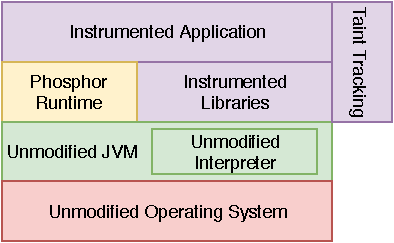
\includegraphics[scale=1]{images/PhosphorArchitecture.pdf}
\caption{\textit{Phosphor's} high-level architecture} \label{phosphorfig}
\end{figure}

It has two main differences from Dytan: 
\begin{itemize}
    \item It does tracking at variable level instead of byte level.
    \item It does not support \textit{implicit information flow} propagation.
\end{itemize}
One big advantage of the first one is that the overhead added is 1x in time and 2-3x in memory consumption. This is a big improvement and makes the tool more viable to be run in real systems. The cost of the much lower overhead is less precision. Tainting at variable level means that \textit{Phosphor} is only able to tell whether a variable is tainted or not, but it is unable to tell exactly which character is causing the attack.
The second difference is more of a limitation, but the authors say that the tool could be extended to support \textit{implicit information flow} propagation.


Although \textit{Phosphor} supports a set of languages and could be easily extended to support Kotlin  as well, it is only portable to languages that run on top of JVM. In this case, \textit{Phosphor} is bound to JVM bytecode, and to port it to a different language, such as PHP, is very difficult. 

\section{SQL parse tree validation} 
\label{sqlparsetree}
SQL parse tree validation \cite{sqlparsetree1,sqlparsetree2} is a type of dynamic analysis where the tool does not need compiled code nor source code, thus being language agnostic. Instead, it puts a \textit{proxy} between the application server and the database. This \textit{proxy} intercepts all the queries to the database and does an \textit{SQL} \textit{parse tree validation}. This way, it can protect applications written in different languages.
\textit{Parse tree validation} consists of building the parse tree of the query and validate it against the parse tree of a known benign query.
Benign queries are then forwarded to the database whilst the malicious ones are dropped. 

Consider the following query \textit{"SELECT 'name' FROM students WHERE id = '12';"} and the parse tree from Figure \ref{invalidparsetree}. When the input is 12 the parse tree is composed only of the green leaves. If a malicious user gives as input the id \textit{"12' OR 1 > 0 --'"}, the parse tree would be composed by the green and red leaves. This way, the tool detects that the parse tree is different and reports the attack.

Although being an interesting approach for detecting \textit{SQL} and \textit{NoSQL} injection attacks, its scope is limited. We can not apply this technique to detect Cross-site scripting or vulnerabilities in language functions (e.g., PHP code injection).


\begin{figure}[h]
\centering
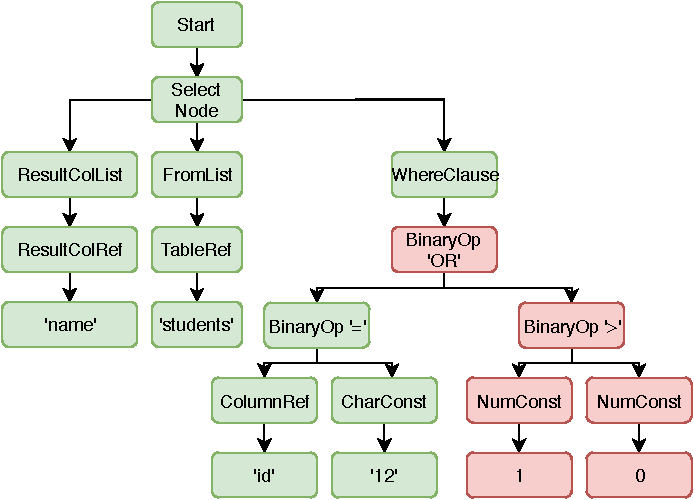
\includegraphics[width =0.8\linewidth]{images/sqlParseTreeInvalid.pdf}
\caption{SQL query parse tree} \label{invalidparsetree}
\end{figure}



\section{Summary}
This chapter first introduced a list of injection vulnerabilities considered in this work. Then, it presented a few static and dynamic approaches at detecting vulnerabilities. % file "Thesis_Background.tex"
\cleardoublepage

%%%%%%%%%%%%%%%%%%%%%%%%%%%%%%%%%%%%%%%%%%%%%%%%%%%%%%%%%%%%%%%%%%%%%%%%
%                                                                      %
%     File: Thesis_Implementation.tex                                  %
%     Tex Master: Thesis.tex                                           %
%                                                                      %
%     Author: Andre C. Marta                                           %
%     Last modified :  2 Jul 2015                                      %
%                                                                      %
%%%%%%%%%%%%%%%%%%%%%%%%%%%%%%%%%%%%%%%%%%%%%%%%%%%%%%%%%%%%%%%%%%%%%%%%

\chapter{The \toolname{} Tool}

%%%%%%%%%%%%%%%%%%%%%%%%%%%%%%%%%%%%%%%%%%%%%%%%%%%%%%%%%%%%%%%%%%%%%%%%

\label{solution}
In this chapter we explain in-depth our approach at solving the complex problem of developing a portable static taint analyzer. Our solution, besides being portable, also aims to be able to perform a context-aware analysis, being as sound and complete as possible.

As stated before, static analyzers are most often bound to a single language and depend on every detail of that language. However, there are a lot of similarities between programming languages, and our approach explores just that. If we take a look at the top trending languages in 2020, ranked by IEEE Spectrum \cite{cass2020top}, used to build web applications, we can divide them in two categories:

\begin{enumerate}
    \item Dynamically typed - Languages that do not check or enforce type-safety at compile-time \cite{tratt2009dynamically}. Instead, type-checking is done during runtime (e.g., Python, JavaScript, PHP and Ruby).
    \item Statically typed - Type checking is done at compile-time (e.g., Java, C\#, GO and Dart).
\end{enumerate}


The languages from each category have many similarities between them. Take for instance JavaScript and PHP, which are very common on web applications. Both of them are object-oriented, have methods, functions, attributes, variables, expressions, etc... Even the \textit{control flow statements} are practically the same (e.g., \textit{if, switch, while, for, do while} etc.). Furthermore, the data flow is almost identical, using assignments. 

Now, if we compare Java and C\# the same is true. Moreover, even comparing languages between categories (e.g., Java and PHP) we see that many of their features overlap. The main difference is that we know the types when analyzing the source code. So from our studies, we found out that when it comes to static taint analysis, we can abstract almost any web programming language. 

With this in mind, our approach introduces a new way of building static analyzers, which consists of having a simple, generic AST (\astname{}) that can represent the structure of the source code of a large set of languages found in web applications. The \astname{}, similarly to the micro-grammars approach \cite{microgrammars}, does not depend on every detail of the languages. Instead, it only represents what is absolutely needed to perform a data flow analysis (in our case, static taint analysis). Section \ref{genericast} explains the abstractions that were made to build the \astname{}.

With the addition of the \astname{}, our analysis gains an extra step comparing to traditional tools. Usually, analyzing a program consists of first parsing the source code and then traversing the resulting AST to find vulnerabilities. By contrast, our approach adds a new, additional step, which consists of converting the source code AST to a \astname{}. Then, we perform the taint analysis on the \astname{} to detect vulnerabilities in the code. This way, the module that performs the taint analysis is completely independent of the language being analyzed. 

Next, we describe the architecture and data flow of \toolname{}. Then, we present the  structure of the \astname{} and how to build it. Finally, we discuss the features of our taint analysis and the compromises and choices that were made.


\section{Architecture and Data Flow}
\label{architecture}


In order to implement a tool that can support several languages simultaneously, we need a decoupled and modular architecture. The architecture of \toolname{}, represented in figure \ref{architecture}, consists mainly of four modules: \textit{Parser}, \textit{AST Converter}, \textit{\astname{} Builder} and \textit{Taint Analyzer}.

\subsection{Parser} 

This module takes as input the source code and produces a source code AST, specific to the language. This module is language-dependent, meaning that every time we add a new language, we need a new parser for that language. Since parsing a full-blown language is a complex task, we delegate it to ANTLR4, which is a widely used parser generator that uses \textit{LL} for parsing \cite{antlr4book}. ANTRL4 has a big community and provides grammars under the MIT license for virtually any language. This way, thanks to ANTRL4, our parsers consist simply of generated code. Furthermore, ANTRL4 also generates tree walkers, which we use to traverse the AST.

\subsection{AST Converter}
Module responsible for traversing the source code AST using the generated tree walker and raising events to the \textit{\astname{} Builder} (e.g., entering and exiting class, methods or functions declarations). These events allow the \textit{\astname{} Builder} to create the \astname{}. This module is the only one needed to program whenever adding support for a new language.

\subsection{\astname{} Builder} 

Module that reacts to the events from the \textit{AST Converter} and internally builds the \astname{}. Section \ref{buildgenericast} shows more in-depth the process of building the \astname{}. 

\subsection{Taint Analyzer} 
Module that takes as input the \astname{} from the \textit{\astname{} Builder} and a configuration file. Then, it traverses the \astname{} using a visitor and propagates the taint marks to find vulnerabilities according to the configuration file. 
Listing \ref{settings} shows an example of a configuration file. In this file, we can specify the value of several parameters, such as:
\begin{itemize}
    \item Source code location - we can set the directory where the source code is and the file extensions that we want to analyze (lines 2, 3)
    \item Entry points - the file and the function where the data flow propagation should start. In the example, it corresponds to lines 6-14, where the entry point is a function called \textit{functionEntryPoint} from the class \textit{EntryPointClass} in the file \textit{EntryPointClass.java}. We also specify which arguments are \textit{tainted}: \textit{"taintedArg","userInput"}
    \item Sensitive functions - functions that when called with \textit{tainted} arguments may result in a vulnerability. In the example we specify a function named \textit{executeQuery} from the class \textit{Statement} (lines 15-20)
    \item Sanitization functions - functions that perform input sanitization and whose return value is always \textit{untainted}. In listing \ref{settings} we configure a sanitization method called \textit{sanitizeInputMethod} from the class \textit{SanitizerClass}
    \item Loops settings - number of times we should analyze a loop. We explain this choice more in-depth in section \ref{loops}.
\end{itemize}


\begin{lstlisting}[
    showstringspaces=false,
    caption={Example of file settings},
    label=settings, float]
{
    "directoryPath": "path/to/app",
    "fileExtension": ".java",
    "numberOfTimesToAnalyzeCycles" : 2,
    "specification": {
        "filename": "EntryPointClass.java",
        "function": {
            "name": "functionEntryPoint",
            "type": "EntryPointClass"
        },
        "taintedVarsOrArgs": [
            "taintedArg",
            "userInput"
        ],
        "sensitiveFunctions": [
            {
                "name": "exectuteQuery",
                "type": "Statement"
            }
        ],
        "sanitizationFunctions": [
            {
                "name": "sanitizeInputMethod",
                "type": "SanitizerClass"
            }
        ],
        "returnTaintedIfTaintedSource": true,
        "taintedAttributes": [
            "taitedAttributeName"
        ]
    }
}
\end{lstlisting}


After traversing the \astname{}, \toolname{} produces a vulnerability report in JSON format. Listing \ref{report} shows an example of a report when analyzing listing \ref{pathpropagation}. In the report, \toolname{} presents the vulnerabilities and the time that took to analyze the program. Furthermore, for each vulnerability it presents a list of conditions that need to be met to reproduce the vulnerability. 

\begin{lstlisting}[
    showstringspaces=false,
    caption={Vulnerability report when analyzing listing \ref{pathpropagation}},
    label=report, float]
{
    "vulnerabilities": [
        {
            "file": "EntryPointClass.java",
            "line": 7,
            "vulnerableMethod": "executeQuery",
            "functionCallStack": [],
            "conditions": [
                {
                    "line": 2,
                    "condition": "input != null"
                },
            ]
        }
    ],
    "timeToProcessMilliseconds": 2074
}
\end{lstlisting}


\begin{figure}[hbt!]
    \centering
    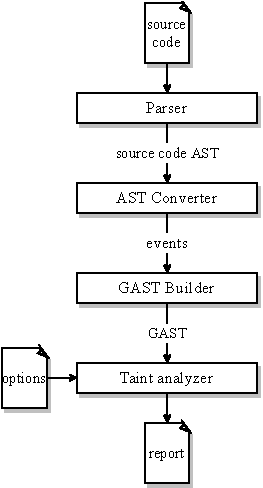
\includegraphics[width =0.4\linewidth]{images/yasat-architecture.pdf}
    \caption{\toolname{} - data flow and architecture overview} 
    \label{architecture}
\end{figure}

\section{\astname{}}
\label{genericast}
Similarly to the micro-grammars solution \cite{microgrammars}, the \astname{} aims to be an intermediate structure that does not depend on every detail of any language. Instead, it abstracts most of the complexity by using generic statements. Each generic statement has a correspondence with a concrete statement of almost any programming language. In this section we describe the structure of the \astname{} by presenting every element that can be part of it. 

\subsection{Elements}

\subsubsection{Constant} 
Element that comprises \textit{strings}, \textit{integers}, \textit{floats}, \textit{null} values etc. Basically, everything that is directly hardcoded in the source code is considered a constant. Since this element never changes, it is impossible to be \textit{tainted}. Figure \ref{constant} presents the \astname{} representation of a constant.

\begin{figure}[hbt!]
    \centering
    \begin{forest}
        [Constant [\textit{value}] ]
    \end{forest}  
    \caption{\astname{} representation of a constant}\label{constant}
\end{figure}


 
\subsubsection{Variable}

This element abstracts, as the name says, the variables in the code. Contains the name of the variable, and if the language is statically typed, it also contains the type of the variable. It can become \textit{tainted} through assignments. Figure \ref{variable} shows the \astname{} representation of a variable.

\begin{figure}[hbt!]
    \centering
    \begin{forest}
        [Variable 
            [\textit{name}]
            [\textit{type}]
        ]
    \end{forest}  
    \caption{\astname{} representation of a variable}\label{variable}
\end{figure}


\subsubsection{Attribute} 
Represents an attribute in a class. It has a name and a type. Also, it can be \textit{tainted}. It is very similar to a variable, as we can see in its representation from figure \ref{attribute}. In our implementation an attribute is a subtype of \textit{Variable}.

\begin{figure}[hbt!]
    \centering
    \begin{forest}
        [Attribute 
            [\textit{name}]
            [\textit{type}]
        ]
    \end{forest}  
    \caption{\astname{} representation of an attribute}\label{attribute}
\end{figure}

\subsubsection{Parameter} Element that abstracts the parameters of methods and functions. It can be \textit{tainted} if it is the parameter of the entry point function, or if the argument passed to a function is \textit{tainted}. Just like the \textit{attribute}, it is also a subtype of \textit{variable}. Figure \ref{parameter} presents its \astname{} representation. 

\begin{figure}[hbt!]
    \centering
    \begin{forest}
        [Parameter 
            [\textit{name}]
            [\textit{type}]
        ]
    \end{forest}  
    \caption{\astname{} representation of a parameter}\label{parameter}
\end{figure}

\subsubsection{Expression} 
Represents a generic abstraction of any expression (e.g., arithmetic, logical, bitwise, comparison etc.). It consists of a list of expressions.
Take for instance the listing \ref{javaexpression} where to each variable, \textit{a, b, c} we assign an expression. In our representation, all these expressions are equal. They all consist of an expression containing two members: a variable named \textit{"x"} and a constant with value \textit{"5"}. This allows us to abstract any operator due to the fact that in data flow analysis, operators (except the assignment operators) do not influence \textit{taint} propagation. For instance, if the variable \textit{x} in listing \ref{javaexpression} is \textit{tainted}, then, all variables will be \textit{tainted}, regardless of their operator.

\begin{lstlisting}[language=Java,
    showstringspaces=false,
    caption={Expression assignment examples},
    label=javaexpression]
boolean a = x == 5;
int b = x + 5;
int c = x * 5;
\end{lstlisting}


\begin{figure}[hbt!]
    \centering
    \begin{forest}
        [Expression 
            [\textit{members}
                [Variable 
                    [\textit{name} [x]]
                    [\textit{type} [int]]
                    ]
                [Constant [\textit{value} [5]]]
            ]
        ]
    \end{forest}  
    \caption{\astname{} representation of the expressions from listing \ref{javaexpression}}\label{expression}
\end{figure}


Since an expression consists only of a list of other expressions, the \textit{taint} propagation is a result of a logical OR of all elements in the expression. Meaning that if any element in the list is \textit{tainted}, the whole expression is marked as \textit{tainted}. 





\subsubsection{Function Call} This element is a subtype of \textit{expression} with the difference that it has a name, referencing the function it is invoking. The arguments are just a list of expressions that can contain anything. Figure \ref{funccall} shows the \astname{} representation of a function call.

\begin{figure}[hbt!]
    \centering
    \begin{forest}
        [Function Call 
            [\textit{name}]
            [\textit{members}]
        ]
    \end{forest}  
    \caption{\astname{} representation of a function call}\label{funccall}
\end{figure}

For instance, the function call \textit{executeQuery(getQuery("name"))} is named \textit{executeQuery} and has as argument another function call named \textit{getQuery}. The latter having as argument a constant with value \textit{"name"}. Figure \ref{funccall1} represents the described tree.

\begin{figure}[hbt!]
    \centering
    \begin{forest}
        [Function Call 
            [\textit{name} [executeQuery]]
            [\textit{members} 
                [Function Call 
                    [\textit{name} [getQuery] ]
                    [Constant [\textit{value} [name]]]
                ]
            ]
        ]
    \end{forest}  
    \caption{\astname{} representation of \textit{"executeQuery(getQuery("name")"}}\label{funccall1}
\end{figure}


A function call is considered \textit{tainted} if any of the following conditions is true: 
\begin{itemize}
    \item the called function is in the source code and it returns a \textit{tainted} value
    \item the called function is in a library and any of its arguments is \textit{tainted}
\end{itemize}

This element also represents method calls that do not have an object as a source (e.g., methods from the same class or any superclass that are not preceded by the keywords \textit{this} or \textit{super} in Java).

\subsubsection{Assignment} 
Statement that represents, as the name indicates, an assignment. Consists of two expressions, one on the left-hand side and another on the right-hand side. It is the main way of propagating \textit{taint} marks. Whenever the expression assigned on the right is evaluated as \textit{tainted}, the mark is also propagated to the expression on the left. Usually, the expression on the left-hand side is just a variable. Listing \ref{javaexpression} contains examples of assignment statements and figure \ref{assignment} shows the \astname{} representation of an assignment.


\begin{figure}[hbt!]
    \centering
    \begin{forest}
        [Assignment
            [\textit{left} 
                [Variable 
                    [\textit{name} [a]]
                    [\textit{type} [boolean]]
                ]
            ]
            [\textit{right} 
                [Expression 
                    [\textit{members}
                        [Variable 
                            [\textit{name} [x]]
                            [\textit{type} [int]]
                            ]
                        [Constant [\textit{value} [5]]]
                    ]
                ]
            ]
        ]
    \end{forest}  
    \caption{\astname{} representation of \textit{"boolean a = x == 5;"}}\label{assignment}
\end{figure}

\subsubsection{Return} This statement, represented in figure \ref{return}, represents the end of the data flow in a path. The returned value is represented by an \textit{expression} which can be \textit{tainted}.

\begin{figure}[hbt!]
    \centering
    \begin{forest}
        [Return 
            [\textit{expression}]
        ]
    \end{forest}  
    \caption{\astname{} representation of a return statement}\label{return}
\end{figure}


\subsubsection{Throw} 
Statement very similar to the return statement. The only difference is that when a return statement is found in the callee function, the data flow is transferred to the caller function. Whilst in the case of a throw statement, the data flow is transferred to a catch block. The thrown expression can be \textit{tainted}. Figure \ref{throw} shows the \astname{} representation of the throw statement.  

\begin{figure}[hbt!]
    \centering
    \begin{forest}
        [Throw 
            [\textit{expression}]
        ]
    \end{forest}  
    \caption{\astname{} representation of a throw statement}\label{throw}
\end{figure}



\subsubsection{Method Call}  
Element that represents method calls. It consists of a source, which can be an object or a class (if the method is static). Listing \ref{methodcall} shows examples of method calls where the source is an object and a class respectively. Figure \ref{methodcallex} shows the \astname{} representation of the first example of listing \ref{methodcall}.

\begin{lstlisting}[language=Java,
    showstringspaces=false,
    caption={Method call examples},
    label=methodcall, float]
context.getUsers();
MyClass.myStaticMethod();
\end{lstlisting}

\begin{figure}[hbt!]
    \centering
    \begin{forest}
        [Method Call
            [\textit{source}
                [Variable 
                    [\textit{name} [context]]
                    [\textit{type} [UserContext]]
                ]
            ]
            [\textit{call} 
                [Function Call
                    [\textit{name} [getUsers]]
                ]
            ]
        ]
    \end{forest}  
    \caption{\astname{} representation of \textit{"context.getUsers();"}}\label{methodcallex}
\end{figure}

A method call is \textit{tainted} if any of the following conditions is true:

\begin{itemize}
    \item the method is not in the analyzed code and the source is \textit{tainted}
    \item the method is in the source code and returns a \textit{tainted} value
\end{itemize}







\subsubsection{New} 
Expression that represents an object creation. It is a subtype of \textit{Expression} and works mostly as a function call to the constructor. Figure \ref{new} shows the \astname{} representation of the \textit{new} expression.

In most languages, the constructor has the same name as the class. But in some languages, the name of the constructor is different from the name of the class (e.g., PHP, Python). For these cases, we keep a configuration file with the names. For instance, \textit{new Foo()} in PHP would result in the call of \textit{\_\_construct()} function of the class \textit{Foo}.

\begin{figure}[hbt!]
    \centering
    \begin{forest}
        [New
            [\textit{name}]
            [\textit{members}]
        ]
    \end{forest}  
    \caption{\astname{} representation of a new expression}\label{new}
\end{figure}


\subsubsection{Attribute access} 
Represents a direct access to an object attribute (e.g., \textit{context.myProperty}). Figure \ref{attributeaccess} shows its \astname{} representation.

\begin{figure}[hbt!]
    \centering
    \begin{forest}
        [Attribute access
            [\textit{source}]
            [\textit{name}]
        ]
    \end{forest}  
    \caption{\astname{} representation of an attribute access}\label{attributeaccess}
\end{figure}



\subsubsection{Code block} 
Element that represents a block of code. Consists of a list of statements. Listing \ref{javaexpression} is an example of a code block with three statements and figure \ref{codeblock} shows the \astname{} of listing \ref{javaexpression}.

\begin{figure}[hbt!]
    \centering
    \begin{forest}
        [Code Block
            [\textit{statements}
                [Assignment
                    [\textit{left} 
                        [Variable 
                            [\textit{name} [a]]
                            [\textit{type} [boolean]]
                        ]
                    ]
                    [\textit{right} 
                        [Expression 
                            [\textit{members}
                                [Variable 
                                    [\textit{name} [x]]
                                    [\textit{type} [int]]
                                    ]
                                [Constant [\textit{value} [5]]]
                            ]
                        ]
                    ]
                ]
                [Assignment,
                    [\textit{left} 
                        [Variable 
                            [\textit{name} [b]]
                            [\textit{type} [int]]
                        ]
                    ]
                    [\textit{right} 
                        [...]
                    ]
                ]
                [Assignment
                    [\textit{left} 
                        [Variable 
                            [\textit{name} [c]]
                            [\textit{type} [int]]
                        ]
                    ]
                    [\textit{right} 
                        [...]
                    ]
                ]  
            ]
        ]
    \end{forest}  
    \caption{\astname{} representation of the code block from listing \ref{javaexpression}}\label{codeblock}
\end{figure}



\subsubsection{Conditional statement} 

Element that abstracts loops (e.g., \textit{for, while, do while} etc.). Consists of a code block and a condition, which is an expression. Figure \ref{condstatement} shows its \astname{} representation. 


\begin{figure}[hbt!]
    \centering
    \begin{forest}
        [Conditional statement
            [\textit{expression}]
            [\textit{code block}]
        ]
    \end{forest}  
    \caption{\astname{} representation of a conditional statement}\label{condstatement}
\end{figure}


\subsubsection{Try Catch} 
Statement composed of a \textit{try} code block, a list of \textit{catch} code blocks and one \textit{finally} code block.
Figure \ref{trycatch} shows its \astname{} representation.



\begin{figure}[hbt!]
    \centering
    \begin{forest}
        [Try Catch
            [\textit{try} [Code Block]]
            [\textit{catch} 
                [Code Block]
                [...]
            ]
            [\textit{finally}[Code Block]]
        ]
    \end{forest}  
    \caption{\astname{} representation of a try catch statement}\label{trycatch}
\end{figure}


\subsubsection{If} Statement that abstracts control flow statements (e.g., \textit{if-else, if-elseif-else} and \textit{switch}). Each option in the control flow has its own code block (e.g., \textit{if-else} has two code blocks - one for \textit{if} and another for the \textit{else}). Figure \ref{ifstmt} shows its \astname{} representation.


\begin{figure}[hbt!]
    \centering
    \begin{forest}
        [If Statement
            [\textit{expression}]
            [\textit{code block}]
            [\textit{else ifs} 
                [If Statement]
                [...]
            ]
            [\textit{else}]
        ]
    \end{forest}  
    \caption{\astname{} representation of an if statement}\label{ifstmt}
\end{figure}

\subsubsection{Function} 
Element that represents a method or a function. It has a name, a return type, a list of parameters and a code block. Its representation can be seen in figure \ref{function}.

\begin{figure}[hbt!]
    \centering
    \begin{forest}
        [Function
            [\textit{name}]
            [\textit{return type}]
            [\textit{parameters} 
                [Parameter]
                [...]
            ]
            [\textit{code block}]
        ]
    \end{forest}  
    \caption{\astname{} representation of a function}\label{function}
\end{figure}


\subsubsection{Class}
This element represents a class in the \astname{}. It has a name, a list of attributes and a list of methods. Furthermore, it can have a superclass, as shown in figure \ref{class}.

\begin{figure}[hbt!]
    \centering
    \begin{forest}
        [Class
            [\textit{name}]
            [\textit{superclass}]
            [\textit{attributes} 
                [Attribute]
                [...]
            ]
            [\textit{methods} 
                [Function]
                [...]
            ]
        ]
    \end{forest}  
    \caption{\astname{} representation of a class}\label{class}
\end{figure}


\subsubsection{File} 
This is the root element of any \astname{}. It has a code block (for languages like PHP or JavaScript), a list of classes, a list of functions and a list of imported files (used to trace calls to imported function). Its structure is represented in figure \ref{file}


\begin{figure}[hbt!]
    \centering
    \begin{forest}
        [File
            [\textit{name}]
            [\textit{code block}]
            [\textit{classes} 
                [Class]
                [...]
            ]
            [\textit{imported files} 
                [File]
                [...]
            ]
        ]
    \end{forest}  
    \caption{\astname{} representation of a file}\label{file}
\end{figure}



One important note to keep in mind is that not every language will use every feature from the \astname{}. For instance, the file element can have statements directly in the root block. Now, this is a feature that it is only used by languages such as PHP and JavaScript. By contrast, Java and C\# do not allow code outside classes, so they do not make use of this feature. 

\subsection{Structure}
As an example of the structure of the \astname{}, consider listings \ref{sametreephp} and \ref{sametreejava}. These listings present code with the exact same functionality written in two different languages (Java and PHP). The code is quite simple -- a class with a method that executes an SQL query given an id. 
Parsing both listings with traditional parsers would result in quite different ASTs, despite the code being very similar. However, when converting the source code ASTs to \astname{}, their representation is almost identical. Figure \ref{sametree} represents the \astname{} from listings \ref{sametreejava} and \ref{sametreephp} where the circled branches only appear in the Java representation since it is statically typed.


\begin{lstlisting}[
        language=php,
        showstringspaces=false,
        caption={MyDbClass in PHP},
        label=sametreephp, float] 
class MyDbClass
{
    function getAddressById($id)
    {
        $sql = "SELECT address FROM users WHERE id = $id";
        return executeSQLQuery($sql);
    }
}
\end{lstlisting}
    
    
\begin{lstlisting}[
    language=Java,
    showstringspaces=false,
    caption={MyDbClass in Java},
    label=sametreejava, float]
public class MyDbClass
{
    public static String getAddressById(String id)
    {
        String sql = "SELECT address FROM users WHERE id =" + id;
        return executeSQLQuery(sql);
    }
}
\end{lstlisting}


    
\begin{figure}[hbt!]
    \begin{forest}
        [File
            [\textit{classes}
                [Class
                    [\textit{methods}
                        [Function
                            [\textit{name}[executeSQLQuery]]
                            [\textit{parameters}
                                [Parameter
                                    [\textit{name}[id]]
                                    [\textit{type},tikz={\node[draw,ellipse,black,fit=()(!1),inner sep=0mm]{};} [String]]
                                ]
                            ]
                            [\textit{return type},tikz={\node[draw,ellipse,black,fit=()(!1),inner sep=0mm]{};}[String]]
                            [\textit{code block}
                                [\textit{statements},l*=3
                                    [Assignment 
                                        [\textit{left}
                                            [Variable
                                                [\textit{name}[sql]]
                                                [\textit{type},tikz={\node[draw,ellipse,black,fit=()(!1),inner sep=0mm]{};}[String]]
                                            ]
                                        ]
                                        [\textit{right}
                                            [Expression
                                                [\textit{members}
                                                    [Constant[\textit{value}[{"SELECT address FROM users WHERE id ="}]]]
                                                    [Variable[\textit{name}[id]]]
                                                ]
                                            ]
                                        ]
                                    ]
                                    [Return 
                                        [\textit{expression}
                                            [FunctionCall
                                                [\textit{name}[executeSQLQuery]]
                                                [\textit{members}[Variable[\textit{name}[id]]]]
                                            ]
                                        ]
                                    ]
                                ]
                            ]      
                        ]
                    ]
                    [\textit{name}[MyDbClass]]  
                ]
            ]
            [\textit{name}[MyDbClass.java]]
        ]
    \end{forest}  
    \vspace*{5mm}
    \caption{\astname{} representing the code from listing \ref{sametreejava} and \ref{sametreephp}} 
    \label{sametree}
\end{figure}




\section{Building the \astname{}}
\label{buildgenericast}

In order to build the \astname{}, we first parse the source code using a parser generated by ANTLR4 to obtain the source code AST. Then, we convert the AST to the \astname{} representation. To do this, we use a tree walker also generated by ANTLR4. The tree walker, which conceptually is a visitor, traverses every node of the AST and for each node it invokes a function when it enters or exits that node. So, in order to convert the AST to \astname{} we need to override some of these methods in the \converter{} to pass state to the \textit{\astname{} Builder}. This is due to the fact that the \textit{\astname{} Builder} keeps the current context in a stack and these methods indicate what is the new context to push and when to pop it. This way the \converter{} is just a class that overrides a set of methods from the generated tree walker. 

Listing \ref{funccallconvertexample} shows part of the PHP \converter{}. In the example, we override two methods from the generated tree walker. The first method is invoked when the tree walker enters a \textit{Func} node and the second when it exits the same node. So, when the tree walker reaches a \textit{Func} node, it invokes the method \textit{enterFunc} from the \converter{}. The latter then invokes a method from the \textit{\astname{} Builder} that pushes the function element to the stack. This way, the \textit{\astname{} Builder} is able to keep track of the context. For instance, if the tree walker encounters a \textit{Parameter} node while in the \textit{Func} node, the parameter would be added to the element on the top of the stack, which in this case would be a function. The function is then popped from the stack when tree walker exits the \textit{Func} node, invoking the method \textit{exitFunc} which calls a method from the \textit{\astname{} Builder} that pops the function (line 8). 

\begin{lstlisting}[language=Java,
    showstringspaces=false,
    caption={Function declaration example},
    label=funccallconvertexample, float]
@Override
public void enterFunc(FuncContext ctx) {
    gastBuilder.addFunction(ctx, ctx.name());
}

@Override
public void exitFunc(FuncContext ctx) {
    gastBuilder.exitFunctionOrMethodDeclaration();
}
\end{lstlisting} 

One important note is that we only push to the stack statements (e.g., functions, classes, assignments, conditional statements, etc.), which are nodes in the AST, while elements such as variables, constants or parameters are not pushed. This is due to the fact that they represent leaves in the AST, so they would be pushed and popped right away. This simplification allows us to override less methods from the tree walker when writing the \converter{} (e.g., we do not need to override \textit{exitVariable}).


Let us now consider listing \ref{assignmentconvertexample} where line 1 corresponds to the assignment being built and lines 3-9 to the sequence of calls made by the \converter{} to the \textit{\astname{} Builder}. Due to lack of space, the signatures of the overridden methods are omitted. When the tree walker enters the assignment, the \converter{} calls a method that adds an assignment to the stack (line 3). Next, it enters a variable and since the assignment is on the top of the stack, the variable becomes the left side of the assignment (line 4). Then, the tree walker enters the expression \textit{"x == 5"} and the \converter{} calls a method that adds an expression to the stack (line 5). After that, it enters a variable and later a constant, which will both be added to the expression, since it is the top of the stack (lines 6, 7). Finally, the tree walker first exits the expression and then the assignment, calling \textit{exitStatementOrExpression} twice (lines 8, 9). Figure \ref{assignment} represents the resulting \astname{} and figure \ref{stacks} represents the stack states when building the tree.

\begin{lstlisting}[language=Java,
    showstringspaces=false,
    caption={Assignment build call sequence},
    label=assignmentconvertexample, float]
boolean a = x == 5;

gastBuilder.addAssignment(ctx);
gastBuilder.addVariable(ctx.VarName());
gastBuilder.addExpression(ctx);
gastBuilder.addVariable(ctx.VarName());
gastBuilder.addConstant(ctx.getText());
gastBuilder.exitStatementOrExpression();
gastBuilder.exitStatementOrExpression();
\end{lstlisting}


\begin{figure}[hbt!]
    \subcaptionbox{}[.333\linewidth]
    {\begin{tikzpicture}
        \selectcolormodel{gray}
        \cell[fill=none]{Assign}
        \stacktop[fill=none]{}
    \end{tikzpicture}}
    \subcaptionbox{}[.333\linewidth]
    {\begin{tikzpicture}
        \cell[fill=none]{Assign [Var a]}
        \stacktop[fill=none]{}
      \end{tikzpicture}}      
      \subcaptionbox{}[.333\linewidth]
    {\begin{tikzpicture}
        \cell[fill=none]{Assign [Var a, Expr]}
        \cell[fill=none]{Expr}
        \stacktop[fill=none]{}
    \end{tikzpicture}}
    \subcaptionbox{}[.333\linewidth]
    {\vspace*{5mm}\begin{tikzpicture}
        \cell[fill=none]{Assign [Var a, Expr]}
        \cell[fill=none]{Expr [Var x]}
        \stacktop[fill=none]{}
    \end{tikzpicture}}
    \subcaptionbox{}[.333\linewidth]
    {\vspace*{5mm}\begin{tikzpicture}
        \cell[fill=none]{Assign [Var a, Expr]}
        \cell[fill=none]{Expr [Var x, Const y]}
        \stacktop[fill=none]{}
    \end{tikzpicture}}
    \subcaptionbox{}[0.333\linewidth]
    {\vspace*{5mm}\begin{tikzpicture}
        \cell[fill=none]{Assign [Var a, Expr]}
        \stacktop[fill=none]{}
    \end{tikzpicture}}    

    \vspace{5mm}
    \caption{Stack state when executing code from listing \ref{assignmentconvertexample}}\label{stacks}
\end{figure}


Converting the AST is as simple as identifying the methods needed to override from the generated tree walker, and then call the functions from the \textit{\astname{} Builder}.
For example, the converter for PHP has 67 lines of code (counting only statements), and from these 67 statements, there are 29 that are different, meaning that a lot of the functions invoked are the same (e.g., \textit{exitStatementOrExpression} is invoked 23 times). 


\section{Analysis features}
\label{analysisfeatures}
Our approach is to use a context-aware static taint analysis to find all potential security vulnerabilities. To be able to statically find vulnerabilities, it is necessary to know what \textit{objects} each variable may refer to, a general problem known as \textit{pointer}, \textit{points-to} or \textit{alias analysis}\cite{sridharan2013alias}. Also, the tool must perform a \textit{path aware} \textit{taint} propagation. Furthermore, it must be able to detect function/method calls between different files.

Next, we discuss the importance of the \textit{alias analysis}. Then, we present our solution to a \textit{path aware} analysis and the method \toolname{} uses to find function/method calls from different files. Finally, we describe our approach to handle loops.

\subsection{Pointer information} 
To illustrate the importance of pointer information, consider the example from listing \ref{pointer}. Assume that \textit{param} is tainted and that \textit{executeQuery} is a sensitive function. In this example, a more conservative approach may assume that \textit{buf1} and \textit{buf2} may reference the same object, thus marking both calls to \textit{executeQuery} as tainted. Instead, \toolname{} traces the data flow through assignments made in each execution path. Thus, being able to identify that line 9 is a safe call and line 13 is a vulnerability.


\begin{lstlisting}[
    language=Java,
    showstringspaces=false,
    caption={Taint propagation example},
    label=pointer, float] 
String param = req.getParameter("name");
StringBuffer buf1;
StringBuffer buf2;

...

buf1.append(param);
String query = buf2.toString();
con.executeQuery(query);

buf2 = buf1;
query = buf2.toString();
con.executeQuery(query);
\end{lstlisting}

Pointer analysis has been subject of much compiler research over the last decades \cite{spath2016boomerang,hind2001pointer}. Since determining what heap object a given variable may point to is undecidable, our approach computes only an approximation based on the data flow through assignments. Meaning that, in much more complex cases, when \toolname{} is unsure to which reference an object is pointing to, it assumes that they all point to the same instance.


\subsection{Path Analysis} In order to perform a precise static taint analysis it is very important to be able to track the data through different paths, ideally all of them. However, in practice, it is almost impossible since static path analysis is a very complex problem. The path is often decided at runtime due to features like \texttt{instanceof}, dynamic dispatch or reflection in Java \cite{hammer2008static}. Furthermore, these features differ between languages. Because of this, we can not have the most precise path analysis for each language. Instead, we perform an approximate path analysis based only on the \textit{control flow statements}, ignoring their conditions. This means that we only look at the structure of the code, and for each conditional statement we propagate the data flow twice: one assuming that the flow enters that path and another assuming it does not. This assumption has the disadvantage of propagating \textit{taint} marks through impossible paths.

Consider now the example from listing \ref{pathpropagation} and assume that the variable \textit{input} is \textit{tainted}. Observing the code, we can easily identify an SQL injection vulnerability at line 7, since at line 3 the \textit{query} is concatenated with the \textit{input}.
In this example, \toolname{} propagates the \textit{taint} marks through two paths: the first executing the \textit{if} and the second the \textit{else}. Finally, it reports the vulnerability at line 7. Also, it mentions that this vulnerability only happens if the expression \textit{"input != null"} at line 2 is true. In more complex cases, for each vulnerability \toolname{} returns the call stack and the conditions that need to be met.

\begin{lstlisting}[
    language=Java,
    showstringspaces=false,
    caption={Path propagation example},
    label=pathpropagation, float] 
String query = "SELECT * FROM users WHERE name=";
if (input != null){
    query = query + input;
} else {
    query = query + "Bob";
}
con.executeQuery(query);
\end{lstlisting}

Let us now consider the example from listing \ref{pathpropagation1}. This example is almost identical to listing \ref{pathpropagation}, with the exception of line 2. This assignment makes the instruction from line 4 unreachable, meaning that in practice, the code has only one possible path. However, \toolname{} has exactly the same output as the previous example: two paths and one vulnerability. This is due to the fact that \toolname{}, and static analysis tools in general, struggle with detecting whether a condition can be true or not.

\begin{lstlisting}[
    language=Java,
    showstringspaces=false,
    caption={Path propagation example with unreachable branch},
    label=pathpropagation1] 
String query = "SELECT * FROM users WHERE name=";
input = null;
if (input != null){
    query = query + input;
} else {
    query = query + "Bob";
}
con.executeQuery(query);
\end{lstlisting}

This way, we perform an approximate path analysis based on the \textit{control flow statements} and their code blocks. The advantage of this kind of path detection is that it can be applied to any language. Furthermore, from our testing, most of the times it is enough to detect vulnerabilities, even though it is not the most accurate.


\subsection{Cross-file function referencing} 
In the last decades, web applications have become increasingly more complex, consisting of many files. For this reason, in order to perform a precise static analysis, we need to be able to perform \textit{taint} propagation between files. However, languages have different ways of importing code. For instance, Java imports packages, which consist of a set of classes, and PHP imports files directly \cite{rountev2004static,hills2014static}. 

To mitigate this problem, our approach supports two generic ways of importing code:
\begin{enumerate}
    \item File inclusion - usually used by dynamically typed languages, such as PHP, Python and JavaScript. Each file has a list of imported files. When \toolname{} finds a call to a function that is not found in the file, it searches in all imported files for that function. If more than one is found, it analyses all of them.
    
    \item Type tracking - works for most of the object-oriented languages, such as Java and C\#. Consists of checking the type of the target of the method call and then checking if that class is in the source code. If the class is found it tries to find the method. If the method is not found, it goes to the superclass.
\end{enumerate}

From our testing and analysis, most of the times \toolname{} correctly propagates the flow to other functions.


\subsection{Loops Analysis}
\label{loops}
Loops have always been tricky for static analysis tools. This is due to the fact that in many cases it is impossible to know how many times a loop will execute, if any. They are often influenced by the user. For this reason, our tool takes a simplistic approach to deal with loops, which is analyzing each loop twice. This approach helps to mitigate cases where a variable only becomes \textit{tainted} after the first iteration. Either way, for more flexibility we left the value configurable, so we could change it depending on the program we want to analyze. 


\begin{lstlisting}[
    language=php,
    showstringspaces=false,
    caption={Vulnerability in while loop},
    label=whileloop] 
$name = $GET_["name"]    
$query = "SELECT * FROM users WHERE name=" 
while(true){
    mysql_query($query);
    $query += $name;
}
\end{lstlisting}

To illustrate this issue, consider listing \ref{whileloop}. In this example, if the \textit{while} loop executes once, there is no vulnerability. This happens because in the first iteration \textit{\$query} is not \textit{tainted} upon executing \textit{mysql\_query}. However, after executing line 5 once, \textit{\$query} becomes tainted which makes the next call to \textit{mysql\_query} unsafe. By propagating the taint more than once, \toolname{} is able to detect this kind of vulnerability.


%%%%%%%%%%%%%%%%%%%%%%%%%%%%%%%%%%%%%%%%%%%%%%%%%%%%%%%%%%%%%%%%%%%%%%%%%%%%%%%%%%%%%%%%%%%%%%%%%%%%%
%%%%%%%%%%%%%%%%%%%%%%%%%%%%%%%%%%%%%%%%%%%%%%%%%%%%%%%%%%%%%%%%%%%%%%%%%%%%%%%%%%%%%%%%%%%%%%%%%%%%%
%%%%%%%%%%%%%%%%%%%%%%%%%%%%%%%%%%%%%%%%%%%%%%%%%%%%%%%%%%%%%%%%%%%%%%%%%%%%%%%%%%%%%%%%%%%%%%%%%%%%%


\section{Summary}
This chapter presented the \astname{} structure and how it manages to abstract different languages by describing each node that can be part of it. Furthermore, we also introduced the architecture of the \toolname{} tool and its taint analysis features.



 % file "Thesis_Implementation.tex"
\cleardoublepage

%\input{Thesis_new_file} % add new .tex files for new chapters
% \cleardoublepage

%\input{Thesis_new_file} % add new .tex files for new chapters
% \cleardoublepage

%\input{Thesis_new_file} % add new .tex files for new chapters
% \cleardoublepage

%%%%%%%%%%%%%%%%%%%%%%%%%%%%%%%%%%%%%%%%%%%%%%%%%%%%%%%%%%%%%%%%%%%%%%%%
%                                                                      %
%     File: Thesis_Results.tex                                         %
%     Tex Master: Thesis.tex                                           %
%                                                                      %
%     Author: Andre C. Marta                                           %
%     Last modified :  2 Jul 2015                                      %
%                                                                      %
%%%%%%%%%%%%%%%%%%%%%%%%%%%%%%%%%%%%%%%%%%%%%%%%%%%%%%%%%%%%%%%%%%%%%%%%

\chapter{Evaluation}
\label{chapter:results}

This chapter presents the results of our taint analysis. We discuss the ability of \toolname{} to detect vulnerabilities and the effort needed to add support for new languages. Finally, we talk about some limitations that our implementation has.

\section{Experimental Evaluation}
\label{evaluation}
The objective of this section is to show that \toolname{} is capable of finding vulnerabilities in web applications written in different languages and that the effort needed to add a new language to the tool is relatively small. First, we present the results of analyzing several web applications in Java and PHP. Then, we discuss the effort needed to add support for another language.


\subsection{Taint analysis tests}
In order to show the ability of \toolname{} to analyze and find vulnerabilities in web applications, we tested \toolname{} against two types of web applications. First, we chose 5 open source applications from GitHub that are deliberately insecure, with documented vulnerabilities. The criteria used to choose them was the number of stars that each application has on GitHub, essentially choosing the most known ones. To run the tests, we had to manually identify the entry points and sensitive functions for each application, meaning that we analyzed each application several times, once for each entry point. Second, we also tested \toolname{} against some real-world open-source web applications. Since these applications are much bigger, we tested them automatically assuming that each file is an entry point and tainting the variables that might be influenced by the user (e.g., \$\_GET[*] in PHP). Tables \ref{results} and \ref{results1} show the results of our analysis. The tests were made on a computer with a Ryzen 1600 processor (6 cores, 12 threads at 3.6GHz) and 16GB of RAM. In the data, we only include files with the extension that we analyzed (e.g., *.java and *.php). Furthermore, we excluded comments and blank lines from the line count. 

\begin{table}[htbp]
    \caption{Deliberately insecure web applications}
    \begin{center}
        \begin{spreadtab}{{tabular}{|l|| l | l  |l | l |}}
            \hline
            @ \textbf{Application}  & @\textbf{\#loc}      & @\textbf{Language}      & @\textbf{Files}     & @\textbf{Vulnerabilities found } \\ [0.5ex] 
            \hline\hline   
            @ WebGoat 8             & 13898     & @ Java       & 320        & 11 \\
            \hline
            @ Vulnado               & 423       & @ Java       & 11         & 3 \\
            \hline
            @ Dvja                  & 950       & @ Java       & 21         & 4 \\
            \hline
            @  DVWA                 & 19651     & @ PHP        & 358        & 18 \\
            \hline
            @  OWASP Vwa            & 1018      & @ PHP        & 27         & 17 \\   
            \hline
            @  Vulnerable-node      & 4207      & @ JavaScript & 13         & 5 \\  
            \hline
            @  Dvna                 & 771      & @ JavaScript  & 14         & 0 \\
            \hline  
            @  Vulpy                 & 2373      & @ Python    & 57         & 6 \\
            \hline  
            @  Dvpwa                 & 674      & @ Python    & 21         & 7 \\   [0.5ex]  
            \hline\hline   
            @ \textbf{Total}        & sum(b2:b10) &              &  sum(d2:d10) &  sum(e2:e10) \\
            \hline
        \end{spreadtab}
    \label{results}
    \end{center}
\end{table}


\begin{table}[htbp]
    \caption{Real-world web applications}
    \begin{center}
        \begin{spreadtab}{{tabular}{|l|| l | l  |l | l |}}
            \hline
            @ \textbf{Application}  & @\textbf{\#loc}      & @\textbf{Language}      & @\textbf{Files}     & @\textbf{Vulnerabilities found } \\ [0.5ex] 
            \hline\hline   
            @  SquirrelMail 1.5     & 46214     & @ PHP        & 376         & 0 \\ 
            \hline
            @  PhpMyAdmin           & 224852    & @ PHP        & 728        & 0 \\  [0.5ex]    
            \hline\hline   
            @ \textbf{Total}        & sum(b2:b3) &              &  sum(d2:d3) &  sum(e2:e3) \\
            \hline
        \end{spreadtab}
    \label{results1}
    \end{center}
\end{table}


\toolname{} analyzed 1946 files and 315031 lines of code and managed to find 71 documented vulnerabilities, such as SQL injection, cross-site scripting, command injection and file inclusion. The analysis times were quite low. The application that took the longest to analyze was \textit{PhpMyAdmin} with 82 seconds. However, the analysis times varied a lot depending on the entry point. Meaning that the longer the path through which the data flows, the longer the analysis time.
 
Besides testing \toolname{} against web applications, we also have a set of 81 unit tests, with simple vulnerabilities, that run on each build of the tool. This way we have more confidence when we make a change to the taint analyzer.


In our tests, the tool had 2 false negatives due to string interpolation in PHP. If we have a variable named "\$id", and then we have "echo "\$\{id\}";" \toolname{} does not understand that "id" is referring to variable "\$id", thus treating "id" as a constant.

\toolname{} did not raise any false positives in the applications from table \ref{results}, we may assume that this is due to our conservative taint analysis and to the relatively simple web applications that we have tested. We can not make any assertions about the false positives from the applications from table \ref{results1} since \toolname{} did not report any vulnerabilities and also, we are not aware of any existing vulnerabilities in the versions we tested.





\subsection{Portability}

Since the objective of this work is to support several languages with as little effort as possible, the portability of the tool is also a metric that we tested. To test the portability, we first implemented the tool to support PHP analysis, and then we added support for Java, which is a substantially different language. While adding support for PHP and Java we were also developing the other modules, so it is hard to tell how much time was spent strictly adding support for each language. However, later, after the tool was built, we added support for JavaScript and then Python and we spent roughly 7 hours adding each language. In our opinion, the main challenge when adding support for a new language is identifying which elements from the grammar are important to the analysis. After that, we just have to  write the converter and some unit tests to make sure the converter works properly.

Table \ref{converters} presents the order in which the languages were added, the number of lines of each converter, the number of unique statements and the number of hours spent developing each one of them.
The number of unique statements is meant to show that the converter does not have much logic, it basically consists of calls to the \astbuilder{}. For example, the converter for Java has 108 lines, 30 of which are repeated (e.g., \textit{exitStatementOrExpression()} is invoked 19 times), leaving us with 78 unique statements.

\begin{table}[htbp!]
    \caption{Converters size and implementation effort}
    \begin{center}
        \begin{tabular}{|c|l|l|l|l|}
           \hline
           \thead{Implementation order} & \thead{Language} & \thead{\#loc} & \thead{Unique statements} & \thead{Hours to \\ implement} \\ [0.5ex] 
           \hline\hline
          1 &  PHP & 67 & 49 & --\\

           \hline
           2 & Java & 108 & 78 & --\\
         
           \hline
          3 & JavaScript & 50 & 41 & 7 \\
           \hline
          4 &  Python & 61 & 49 & 7 \\
           \hline
          \end{tabular}
          \label{converters}
    \end{center}
    
\end{table}



\section{Limitations}
\label{limitations}
In this section we present the limitations of our tool. Most of them are related to the nature of static taint analysis, such as propagating the data flow through impossible paths or the pointer analysis problem. Besides the limitations already discussed we also found another related to lambda functions. Since our taint analysis only propagates \textit{taint} marks, we can not track the implementation of lambda functions.
For example, consider listing \ref{lambda}, written in JavaScript, and assume that the \textit{userInput} is tainted. In this case, we have an arrow function (lambda equivalent in JavaScript) \textit{x} that accepts a parameter \textit{query} and then executes this query against the database. This is a very simple program, with only two lines, however, \toolname{} struggles to find the vulnerability from line 3. This flaw is due to the fact that in our implementation, \textit{x} is just a variable, it does not know that \textit{x} is an object that holds a function. Furthermore, this variable \textit{x} could be passed around as an argument to other functions. So, in complex cases, we quickly lose track of \textit{x} and are unable to know what is the implementation of the function that \textit{x} is holding.


\begin{lstlisting}[
    showstringspaces=false,
    caption={JavaScript lambda example},
    label=lambda]
var x = query => db.executeQuery(query);

x.call("SELECT * FROM users WHERE name=" + userInput);
\end{lstlisting}

This problem does not have an easy solution since it would require the tool to precisely track the flow of data in the application, which statically is virtually impossible. % file "Thesis_Results.tex"
\cleardoublepage

%%%%%%%%%%%%%%%%%%%%%%%%%%%%%%%%%%%%%%%%%%%%%%%%%%%%%%%%%%%%%%%%%%%%%%%%
%                                                                      %
%     File: Thesis_Conclusions.tex                                     %
%     Tex Master: Thesis.tex                                           %
%                                                                      %
%     Author: Andre C. Marta                                           %
%     Last modified :  2 Jul 2015                                      %
%                                                                      %
%%%%%%%%%%%%%%%%%%%%%%%%%%%%%%%%%%%%%%%%%%%%%%%%%%%%%%%%%%%%%%%%%%%%%%%%

\chapter{Conclusions}
\label{chapter:conclusions}
In this work, we presented a new approach to static taint analysis that supports the addition of new languages with little programming effort. We were able to achieve this by taking advantage of the fact that the programming languages used in web applications have many similarities between them. With this in mind, instead of analyzing the source code directly, we first parse the source code and then build a generic AST (\astname{}) based on it. After that, we traverse the \astname{} to find vulnerabilities, thus decoupling the analysis from the parsing. The \astname{} does not represent every detail of a language, instead, it contains only what is needed to perform the analysis. This allows it to be able to represent a large set of programming languages used in web applications. The only parts bound to the language being analyzed are the parser, which in our implementation consists of generated code, and the module that converts source code AST into the \astname{}, which is usually less than 110 lines of code. 

The solution was implemented in the \toolname{} tool, using Java with parsers and tree walkers generated by ANTLR4. \toolname{} supports \implangs{} and was tested against several web applications written in different languages. Based on the results of our tests and the number of languages supported, we consider that our goal was successfully achieved.


\section{Future work}

The presented work leaves room for several possible improvements that were not possible to develop due to time constraints. \astname{} could be extended to support even more languages and more features (e.g., adding support for lambda functions). The taint analyzer could also be extended. For instance, we could make it more accurate by using a more precise pointer analysis. Furthermore, we could also track the value of each variable, removing this way the lambda limitation described in section \ref{limitations}.  % file "Thesis_Conclusions.tex"
\cleardoublepage

% ----------------------------------------------------------------------
%  Bibliography
% ----------------------------------------------------------------------

% Add entry in the table of contents as chapter
\phantomsection
\addcontentsline{toc}{chapter}{\bibname}

% Include all references in .bib file, even non-cited ones...
%\nocite{*} % this should be used carefully because it is not correct!

% Produces the bibliography section when processed by BibTeX
%
% Bibliography style
% > entries ordered alphabetically
%\bibliographystyle{plain}
% > unsorted with entries appearing in the order in which the citations appear.
%\bibliographystyle{unsrt}
% > entries ordered alphabetically, with first names and names of journals and months abbreviated
%\bibliographystyle{abbrv}
% > entries ordered alphabetically, with reference markers based on authors' initials and publication year
%\bibliographystyle{alpha}
%
% Replacement bibliography styles provided by 'natbib' package
% (plainnat.bst, abbrvnat.bst, unsrtnat.bst )
% > entries ordered alphabetically
%\bibliographystyle{plainnat}
% > unsorted with entries appearing in the order in which the citations appear.
%\bibliographystyle{unsrtnat}
% > entries ordered alphabetically, with first names and names of journals and months abbreviated
%\bibliographystyle{abbrvnat} % <<<<< SELECT IF USING REFERENCES BY AUTHOR/YEAR
% > entries ordered alphabetically, with reference markers based on authors' initials and publication year
%\bibliographystyle{alpha}
%
% Custom bibliography style adapted from 'natbib' package
%   (based on http://tex.stackexchange.com/questions/5053/is-it-possible-to-get-unsrt-abbrv-bibliography)
%   (unsrtnat.bst + abbrvnat.bst -> abbrvunsrtnat.bst)
%   (original files copied from:
%   http://tug.ctan.org/macros/latex/contrib/natbib/abbrvnat.bst
%   http://tug.ctan.org/macros/latex/contrib/natbib/unsrtnat.bst
% > unsorted with entries appearing in the order in which the citations appear, with first names and names of journals and months abbreviated.
\bibliographystyle{alpha} % <<<<< SELECT IF USING REFERENCES BY NUMBER (CITATION ORDER)  %mpc: changed, was abbrvunsrtnat

% External bibliography database file in the BibTeX format
\bibliography{Thesis_bib_DB} % file "Thesis_bib_DB.bib"

\cleardoublepage

% ----------------------------------------------------------------------
%  Appendix (optional)
%
%  CAUTION: 1) the main document (up to the conclusions) shall not exceed 80 pages
%           2) the document shall not exceed a total of 100 pages (per IST regulations)
% ----------------------------------------------------------------------
\appendix

% add page number prefix according to apendix chapter (optional)
%\renewcommand{\thepage}{\thechapter.\arabic{page}}

% re-set arabic numbering (A.1,A.2,...) (optional, use only if chapter prefix is added)
%\setcounter{page}{1}

% ----------------------------------------------------------------------
\end{document}
% ----------------------------------------------------------------------

